
%  Created by Colin Williams on 2012-01-06.
%  Copyright (c) 2012 __MyCompanyName__. All rights reserved.
%
\documentclass[]{article}

% Use utf-8 encoding for foreign characters
\usepackage[utf8]{inputenc}

% the page geometry.
\usepackage[a4paper,top=2cm, bottom=2cm, left=1cm, right=1cm]{geometry}
\usepackage{minibox}
% Uncomment some of the following if you use the features
%
% Running Headers and footers
%\usepackage{fancyhdr}

% Multipart figures
%\usepackage{subfigure}

% More symbols
%\usepackage{amsmath}
%\usepackage{amssymb}
%\usepackage{latexsym}

% Surround parts of graphics with box
\usepackage{boxedminipage}

% Package for including code in the document
\usepackage{listings}

% If you want to generate a toc for each chapter (use with book)
\usepackage{minitoc}

% This is now the recommended way for checking for PDFLaTeX:
\usepackage{ifpdf}
\usepackage{comment}

%\newif\ifpdf
%\ifx\pdfoutput\undefined
%\pdffalse % we are not running PDFLaTeX
%\else
%\pdfoutput=1 % we are running PDFLaTeX
%\pdftrue
%\fi


\usepackage{array}
\usepackage{url}
\usepackage{listings}
\usepackage{color}
\usepackage{amsmath}
\usepackage{mathtools}

% clickable links in the contents section
\usepackage{hyperref}
\hypersetup{
    colorlinks,
    citecolor=black,
    filecolor=black,
    linkcolor=black,
    urlcolor=black
}


\definecolor{dkgreen}{rgb}{0,0.6,0}
\definecolor{gray}{rgb}{0.5,0.5,0.5}
\definecolor{mauve}{rgb}{0.58,0,0.82}


\newcommand*\vtick{\textsc{\char13}}

\lstset{
  language=Java,
  tabsize=4,
  showstringspaces=false,
  basicstyle=\tt,
  numberstyle=\tiny\color{gray},      % line number style
  keywordstyle=\color{blue},          % keyword style
  commentstyle=\color{dkgreen},       % comment style
  stringstyle=\color{mauve},          % string literal style
}

\ifpdf
\usepackage[pdftex]{graphicx}
\else
\usepackage{graphicx}
\fi

% this gives us \FloatBarrier to prevent images to float all to the end
\usepackage{placeins}
\newcommand\Genius{{\sc Genius}}

% Alter some LaTeX defaults for better treatment of figures:
    % See p.105 of "TeX Unbound" for suggested values.
    % See pp. 199-200 of Lamport's "LaTeX" book for details.
    %   General parameters, for ALL pages:
    \renewcommand{\topfraction}{0.9}	% max fraction of floats at top
    \renewcommand{\bottomfraction}{0.8}	% max fraction of floats at bottom
    %   Parameters for TEXT pages (not float pages):
    \setcounter{topnumber}{2}
    \setcounter{bottomnumber}{2}
    \setcounter{totalnumber}{4}     % 2 may work better
    \setcounter{dbltopnumber}{2}    % for 2-column pages
    \renewcommand{\dbltopfraction}{0.9}	% fit big float above 2-col. text
    \renewcommand{\textfraction}{0.07}	% allow minimal text w. figs
    %   Parameters for FLOAT pages (not text pages):
    \renewcommand{\floatpagefraction}{0.7}	% require fuller float pages
	% N.B.: floatpagefraction MUST be less than topfraction !!
    \renewcommand{\dblfloatpagefraction}{0.7}	% require fuller float pages

	% remember to use [htp] or [htpb] for placement



%===========================================================================
\title{Using the {\Genius} Framework for Running Autonomous Negotiating Parties}
\author{T. Baarslag, W. Pasman, K. Hindriks, D. Tykhonov}

\date{\today}

\begin{document}

\ifpdf
\DeclareGraphicsExtensions{.pdf, .jpg, .tif}
\else
\DeclareGraphicsExtensions{.eps, .jpg}
\fi

\maketitle


\abstract{\noindent {\Genius} \cite{Genius}~is a negotiation environment that implements an open architecture for heterogeneous negotiating parties. {\Genius}~can be used to implement, or simulate, real life negotiations. This document describes how you can install the environment, work with the provided scenarios and negotiation parties, and write, compile, and run an party yourself. \\

\noindent
For a quick start on how to set up your workspace with {\Genius} we refer to Section \ref{sec:appendix}.

}

\pagebreak
\tableofcontents

\pagebreak


%=========================================================================================
\section{Theory Crash Course}
This section provides a crash course on some essential theory needed to understand the negotiation system. Furthermore, it provides an overview of the features of a negotiation implemented in {\Genius}.

\subsection{Bids, Issues and Values}
Parties participating in a negotiation interact in a domain. The domain specifies the possible bids. The parties all have their own preferences, which is reflected in their profile.  Figure~\ref{Fig:domain} shows a picture of a domain that describes the issues in the negotiation.

\begin{figure}[htb]
	\centering
	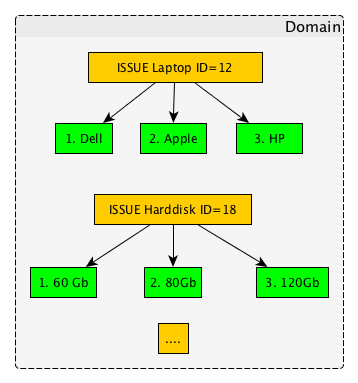
\includegraphics[width=0.4\textwidth]{media/domain.png}
	\caption{An example domain for laptop negotiation. Issues are orange, values are green}\label{Fig:domain}
\end{figure}

The \textit{Domain} describes which issues are the subject of the negotiation and which values an issue can attain. A domain contains $n$ issues: $D=(I_1,\ldots,I_n)$. Each issue $i$ consists of $k$ values: $I_i=(v^i_1,\ldots,v^i_k)$.  Combining these concepts, a party can formulate a \textit{Bid}: a mapping from each issue to a chosen value (denoted by $c$), $b=(v^i_{c},\ldots,v^n_{c})$. 

To give an example, in the laptop domain the issues are ``laptop'', ``harddisk'' and ``monitor''. In this domain the issues can only attain discrete values, e.g. the ``harddisk'' issue can only have the values ``60Gb'', ``80Gb'' and ``120Gb''. These issues are all instance of \textit{IssueDiscrete}. A valid bid in the laptop domain is e.g. \verb|Laptop:Dell, Harddisk: 80Gb, monitor:17"|. A bid \verb|Laptop Asus, Harddisk: 80Gb, monitor:17"| is not a valid bid because Asus is not a valid issue value in the example domain, and \verb|Laptop Asus, Harddisk: 80Gb, CPU:i7"|  is not valid because CPU is not an issue in this domain. 

\subsection{Preference Profile, Utility Space and Elicitation}
The \textit{Preference Profile} describes how bids are preferred over other bids. Typically, each participant in a negotiation has his own preference profile. Genius supports utility spaces and partially ordered profiles.

\subsubsection{Utility spaces}
One form of profile is the \textit{UtilitySpace}. The UtilitySpace specifies the preferences using an \textit{evaluator}: a function that maps bids into a real number in the range [0,1] where 0 is the minimum utility and 1 is the maximum utility of a bid. So a bid is preferred if and only if it has a higher utility than another bid.

A common form of the Utility space is the \textit{Linear Additive Utility Space}. This space is additive because each of the issue values in the domain have their own utility of their own, and all the sub-utilities just add up for the total utility of the bid. For instance, we like Apple with utility evaluation 0.7 and Dell with 0.4, completely independent of how much memory the computer has. Figure~\ref{Fig:utilspace} shows a picture of a utility space for the example domain that we gave above.

\begin{figure}[htb]
	\centering
	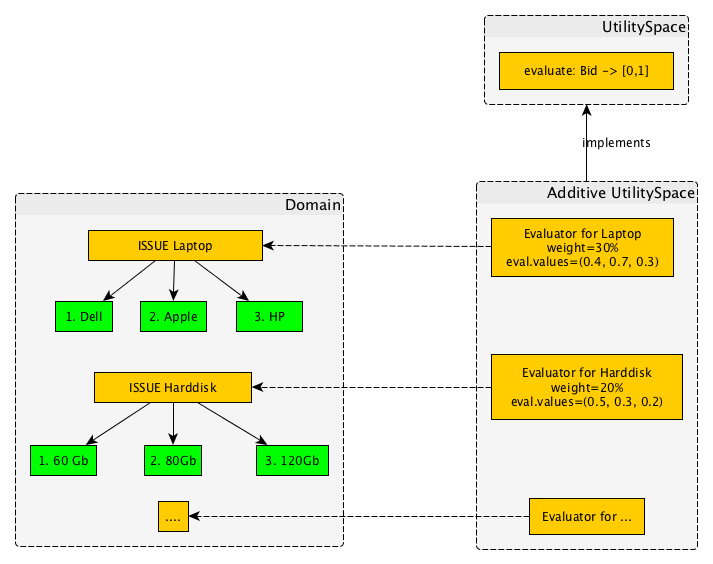
\includegraphics[width=0.6\textwidth]{media/utilspace.png}
	\caption{An example additive utility space for the laptop domain.}\label{Fig:utilspace}
\end{figure}
 
In an additive space the evaluator also specifies the importance of the issue relative to the other issues in the form of a weight. The weights of all issues sum up to 1.0 to simplify calculating the utility of a bid. The utility is the weighted sum of the scaled evaluation values.

\begin{equation}
	U(v^i_{c},\ldots,v^n_{c}) = \sum_{i=1}^{n} w_i \dfrac{\text{eval}(v^i_{c})}{\text{max}(\text{eval}(I_i))}
	\label{eqn:Utility}
\end{equation}

Other types of UtilitySpaces are the \textit{ConstraintUtilitySpace} and the \textit{NonlinearUtilitySpace}. These are more experimental and not described here in more detail.

\subsubsection{Preference Uncertainty through a Partially ordered profile}\label{sec:partialordering}

The \textit{UncertainAdditiveUtilitySpace} is a profile type that uses a partial ordering instead of assigning a utility value to bids. In a partial ordering, the available information is that bid $X$ is preferred over bid $Y$ for a subset of possible bids. 

An UncertainAdditiveUtilitySpace profile is generated from a AdditiveUtilitySpace as will be described in the section \ref{sec:scenariocreation}, but the underlying AdditiveUtilitySpace is normally not visible for the party that uses the profile. Instead, given an UncertainAdditiveUtilitySpace, the agent's goal is to formulate its own estimated utility function $ \hat{U}(\omega) $ that approximates the real utility function $ U(\omega) $ for every bid $\omega$ as much as possible. That is, the agent needs to find `the most likely' utility function from a limited ranking of outcomes.

The generation of the partial ordering works as follows. The values $comparisons$, $errors$ and $experimental$ are additional parameters of the UncertainAdditiveUtilitySpace that control the generation. 
\begin{enumerate}
\item a subset of $comparisons$ bids are selected randomly from all possible bids. 
\item the selected bids are sorted in ascending utility
\end{enumerate}

This partial ordering is available to the agent through what we call a \textit{UserModel}.

Notice: AbstractNegotiatonParty on initialization will do a simplistic attempt to convert an UncertainAdditiveUtilitySpace into an AdditiveLinearUtilitySpace. 

Warning: if the number of possible bids is very large, iterating over all bids in the outcome space and sorting them can result in running out of memory.  

\subsubsection{Elicitation through the User}

In the case where the preference profile is uncertain, the Agent might want to elicit more information about the true utility space in order to improve its UserModel. It is able to do so by querying the \textit{User} against an \textit{elicitation cost}. A User is generated automatically from an UncertainAdditiveUtilitySpace as will be described in section \ref{sec:scenariocreation}. To get a clearer picture of the role of the User, one can think of it as being the personified ``User" for which the agent is negotiating. The Agent can then ask the User questions about what it wants to improve its performance, but this bothers the User to an extent. This bother is captured by the elicitation cost attributed to the User. At the end of the negotiation, the true performance of the Agent is recorded as the User utility. It is obtained by subtracting the total bother inflicted to the User to the utility of the bid agreed upon. Namely, if $\omega$ is the agreement, then:

\begin{equation}
	\text{User Utility}=U(\omega)-\text{Total Bother Cost}
\end{equation}

Figure \ref{Fig:uncertainty} presents an overview of the dynamics between the different actors involved under preference uncertainty.

\begin{figure}[htb]
	\centering
	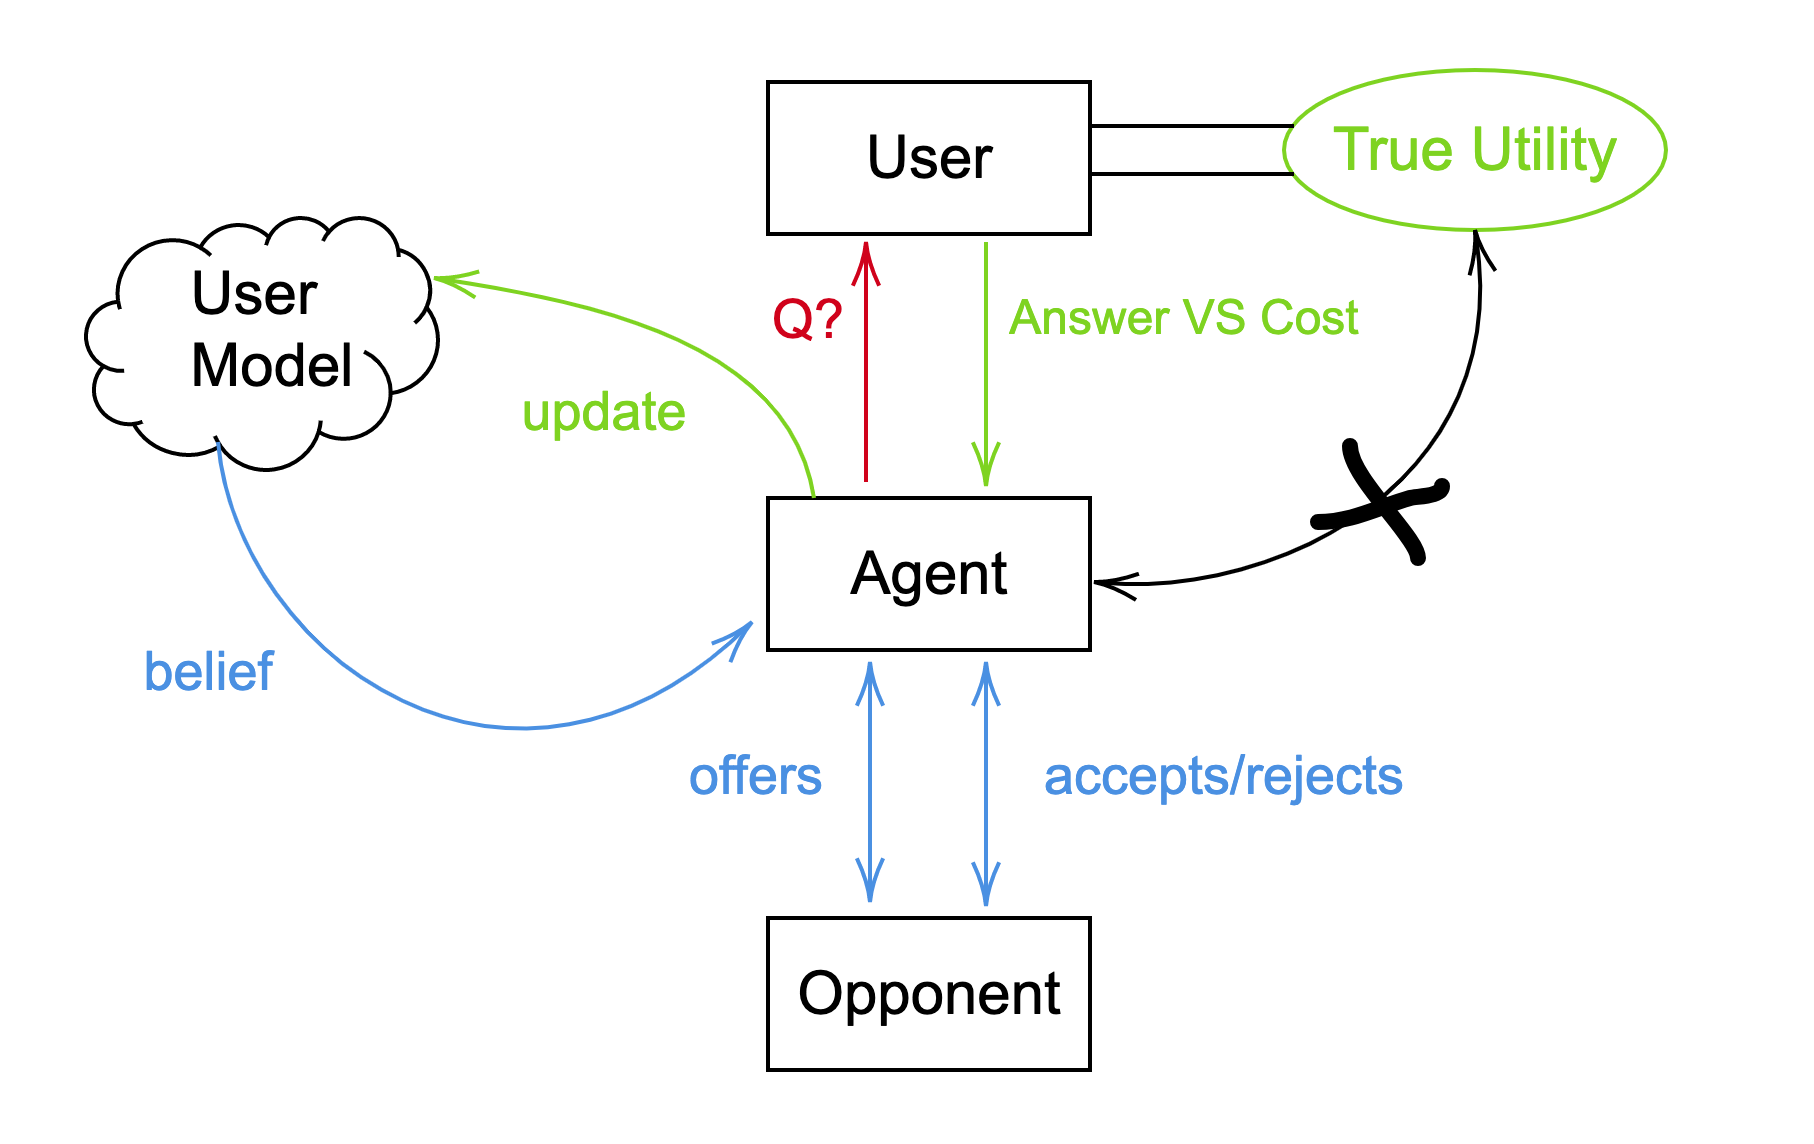
\includegraphics[width=0.6\textwidth]{media/Uncertainty_Diagram.png}
	\caption{Negotiation dynamics under preference uncertainty}\label{Fig:uncertainty}
\end{figure}

\subsection{Optimality of a Bid}
In general, given the set of all bids, there are a small subset of bids which are more preferred as outcomes by all parties in the negotiation. Identifying these special bids may lead to a better agreement for both parties.

For a single party, the optimal bid is the bid that is most preferred / has maximum utility. Often this bid is not preferred so much / has a low utility for other parties, and therefore the chance of agreement is low. A more general notion of optimality of a negotiation involves the utility of all parties.

\begin{figure}[htb]
	\centering
	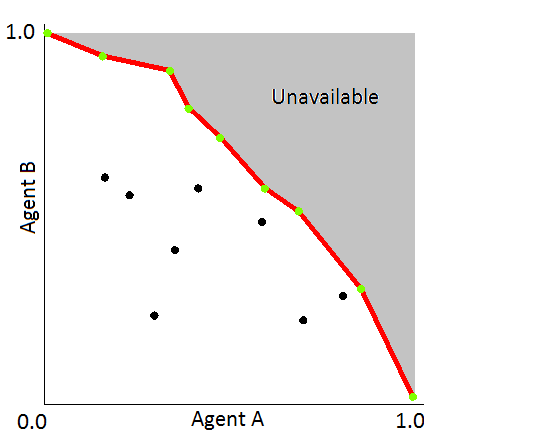
\includegraphics[width=0.37\textwidth]{media/image5.png}
\caption{A point indicates the utility for both parties of a bid. The red line is the Pareto optimal frontier.}\label{Fig:utility plot}
\end{figure}

There are multiple ways to define a more global ``optimum''. One approach to optimality is that a bid is not optimal for both parties if there is another bid that has the higher utility for one party, and at least equal utility for the other party. Thus, only bids in Figure~\ref{Fig:utility plot} for which there is no other bid at the top right is optimal. This type of optimality is called Pareto optimality and forms an important concept in automated negotiation. The collection of Pareto optimal bids is called the Pareto optimal frontier.

A major challenge in a negotiation is that parties can hide their preferences. This entails that an party does not know which bid the opponent prefers given a set of bids. This problem can be partly resolved by building an \textit{opponent model} of the opponent's preferences by analyzing the negotiation trace. Each turn the party can now offer the best bid for the opponent given a set of similar preferred bids. {\Genius}  provides a number of components that can estimate an opponent model.

\subsection{Negotiation Protocol}
The negotiation protocol determines the overall order of actions during a negotiation. Parties are obliged to stick to this protocol, as deviations from the protocol are caught and penalized. {\Genius} supports multiple protocols. These are discussed in detail in section \ref{sec:protocols}.

 
\subsection{Reservation Value}
A reservation value is a real-valued constant that sets a threshold below which a rational party should not accept any offers. Intuitively, a reservation value is the utility associated with the Best Alternative to a Negotiated Agreement (BATNA).

A reservation value is the minimum acceptable utility, offers with a utility would normally not be accepted by a party. Reservation values typically differ for each negotiation party. In case no reservation value is set in a profile, it is assumed to be 0. Notice that if a negotiation ends with no agreement, parties normally get a utility of 0, regardless of the reservation value.

\subsection{Time Pressure}
A negotiation lasts a predefined time in seconds, or alternatively rounds. In {\Genius}~the time line is \emph{normalized}, i.e.: time $t \in [0, 1]$, where $t = 0$ represents the start of the negotiation and $t = 1$ represents the deadline. Notice that manipulation of the remaining time can be a factor influencing the outcome.

There is an important difference between a time-based and rounds-based protocol. In a time-based protocol the computational cost of an party should be taken into account as it directly influences the amount of bids which can be made. In contrast, for a rounds-based negotiation the time can be thought of as paused within a round; therefore computational cost does not play a role.

Apart from a deadline, a scenario may also feature \emph{discount factors}. Discount factors decrease the utility of the bids under negotiation as time passes. While time is shared between both parties, the discount generally differs per party. 
The default implementation of discount factors is as follows: let $d$ in $[0, 1]$ be the discount factor that is specified in the preference profile of a party; let $t$ in $[0, 1]$ be the current normalized time, as defined by the timeline; we compute the discounted utility $U_D^t$ of an outcome $\omega$ from the undiscounted utility function $U$ as follows:
\begin{eqnarray}
U_D^t(\omega) = U(\omega) \cdot d^t
\end{eqnarray}
If $d = 1$, the utility is not affected by time, and such a scenario is considered to be undiscounted, while if $d$ is very small there is high pressure on the parties to reach an agreement. Note that discount factors are part of the preference profiles and therefore different parties may have a different discount factor.

If a discount factor is present, reservation values will be discounted in exactly the same way as the utility of any other outcome. It is worth noting that, by having a discounted reservation value, it may be rational for parties to end the negotiation early and thereby default to the reservation value.

Note: time pressure has little meaning if the profile is not defined in terms of utilities, eg a partially ordered profile.
 
%=========================================================================================
\section{Protocols}\label{sec:protocols}
This section describes the various negotiation protocols. The protocol determines the overall order of actions during a negotiation.
This section focuses on the MultiParty protocols as these have been properly developed. There is also a protocol class for the bilateral negotiation, but this is basically a hard coded Stacked Alternating Offers Protocol and not further developed. 

  The (Multilateral)  protocol describes if the negotiation is finished, what the agreement is, which actions can be done in the next round.   Briefly, to run a session the system checks with the protocol if the negotiation is already finished,  and if not which calls need to be made to the parties (both chooseAction and receiveMessage).  We recommend checking the javadoc of MultilateralProtocol for up-to-date detail information and how the protocol is used by the system to run sessions.
  
 The Multilateral protocol uses the notion of rounds and turns to describe the negotiation layout. A round is a part of the negotiation where all participants get a turn to respond to the current state of the negotiation. A turn refers to the opportunity of one party to make a response to the current state of the negotiation. 
  
If a party violates the protocol -- for instance by sending an action that is not one of the allowed ones, or by crashing, the negotiation ends and the outcome usually is 'no agreement' for all parties.  In bilateral negotiation we have a special case then: the party's utility is set to its reservation value, whereas the opponent is awarded the utility of the last offer.

All protocols are found in the package \verb|genius.core.protocol| and have the names matching the subsections below.


\subsection{Stacked Alternating Offers Protocol}
According to this protocol \cite{MultilateralOffersProtocols} , all of the participants around the table get a turn per round. Turns are taken clock-wise around the table. One of the negotiating parties starts the negotiation with an offer that is observed by all others immediately. Whenever an offer is made, the next party in line gets a call to receiveMessage containing the bid, followed by a call to chooseAction from which it can return the following actions:
\begin{itemize}
\item Accept the offer (not available the very first turn). 
\item send an Offer to make a counter offer (thus rejecting and overriding the previous offer, if there was any) 
\item send an EndNegotiation and ending the negotiation without any agreement.
\end{itemize}

This protocol is the default protocol for Parties (as returned by getProtocol()).


\subsection{Alternating Multiple Offers Protocol}
According to this protocol \cite{MultilateralOffersProtocols}, all parties have a bid from all parties available to them, before they vote on these bids. This implemented in the following way: The protocol has a bidding phase followed by voting phases. In the bidding phase all participants put their offer on the table. These offers appear to all parties through receiveMessage() in a specific order. In the voting phases all participants vote on all of the bids on the negotiation table, in the same order as received. For each offer, the party's chooseAction() is called. If one of the bids on the negotiation table is accepted by all of the parties, then the negotiation ends with this bid. 

In each even round (we start in round 0), each party gets only one turn for an OfferForVoting. 

In each odd round there are N voting turns for each party (N being the number of offers), one for each offer in order of reception. these are the available options:
\begin{itemize}
\item Accept the offer
\item Reject the offer
\end{itemize}


\subsection{Alternating Majority Consensus Protocol}

This protocol is essentially equal to the Alternating Multiple Offers Protocol, but now an offer the protocol keeps track of the acceptable offer that got most accepts.
Initially, this may be the first offer that got one accept. After a number of rounds, some offers receive multiple accepts and these then become the new acceptable offer.

If an offer is accepted by all parties, the negotiation ends. Otherwise, the negotiation continues (unless the deadline is reached). If the deadline is reached, the acceptable offer becomes the agreement.
 
 
\subsection{Simple Mediator Based Protocol}
In this protocol, the parties do not hear the other parties directly. Instead, they only hear the mediator and the mediator hears the bids of all the parties. The mediator determines which bid will be voted on, collects the votes and determines the outcome. The mediator is just another NegotiationParty, but it extends Mediator.

The protocol requires that exactly one party is a Mediator. The {\Genius} GUI enforces this presence of a Mediator. When you run a negotiation from the command line you have to ensure the presence of a single Mediator.

This protocol uses the following turns in every round:
\begin{enumerate}
\item Mediator proposes an OfferForVoting
\item The other parties (not the mediator) place a VoteForOfferAcceptance on the OfferForVoting
\item The mediator makes a InformVotingResult that informs all parties about the outcome of this round.
\end{enumerate}

With this protocol, the last InformVotingResult with an accept determines the current outcome. 

As mentioned, you have to provide one mediator. There is the following options 
\begin{itemize}
\item RandomFlippingMediator.   This mediator generates random bids until all parties accept. Then, it
  randomly flips one issue of the current offer to generate a new offer. It
  keeps going until the deadline is reached. 
 \item FixedOrderFlippingMediator.   This mediator behaves exactly like the RandomFlippingMediator, except that it uses a fixed-seed Random generator for every run. This makes it easier for testing. 

\end{itemize}

\subsection{Mediator  Feedback Based Protocol}
Like the Simple Mediator Based Protocol, the parties do not hear the other parties directly. Instead, they only hear the mediator and the mediator hears the bids of all the parties. The mediator determines which bid will be voted on, collects the votes and determines the outcome. The mediator is just another NegotiationParty, but it extends Mediator.

 The mediator generates its first bid randomly and sends it to the negotiating parties. After each bid, each party compares the mediator\vtick s new bid with his previous bid and gives feedback (`better', `worse' or `same')  to the mediator. For its further bids, the mediator updates the previous bid, hopefully working towards some optimum. The negotiation runs on until the deadline (unless some party crashes). This protocol is explained in detail in \cite{MultiMediatedNegoProtocolsWithFeedback}.

This protocol uses the following turns in every round:
\begin{enumerate}
\item Mediator proposes an OfferForFeedback. 
\item The other parties (not the mediator) place a GiveFeedback,  indicateing whether the last bid placed by the mediator is better or worse than the previous bid.
\end{enumerate}

The accepted bid is the last bid that was not receiving a `worse' vote. 

\subsection{Beyond the Protocol}
This section outlines the procedures for the parts of the session outside the scope of the protocol specification.

Before the protocol can be started, the parties have to be loaded and initialized. During initialization, the party's persistent data may have to be loaded from a file. If the persistent data can not be read, a default empty dataset is created for the party. Then the party's init code is called to set up the party. All the time spent in this initialization phase is already being subtracted from the total available negotiation time.

After the protocol has been completed, the protocol is called a last time to determine the final outcome. 
The parties are called to inform them that the negotiation ended, and what the outcome was. This happens even when parties crashed or did illegal actions. The negotiation has already finished, so these calls are not weighing in on the total negotiation time. Instead, these calls are typically limited to 1 second. 

Finally, if the party has modified the persistent data, this data needs to be saved. Again, this action is limited to a 1 second duration.

Errors surrounding these out-of-protocol procedures are not part of the negotiation itself and therefore logged and handled separately. These errors are printed only to the console/terminal \footnote{To see the console output, run from Eclipse or start up Genius from a separate terminal. }
, and only from the single session runner.


%=========================================================================================
\section{Install and Run {\Genius} }
{\Genius}  can run on any machine running Java 8. Java 9 is not yet supported. Please report any bugs found to \url{negotiation@ii.tudelft.nl}.

To install the environment, the file \texttt{genius-XXX.zip} can be downloaded from \url{http://ii.tudelft.nl/genius/?q=article/releases}. Unzip the file at a convenient location on your machine. This will result in a folder ``genius-XXX" containing the following files:

\begin{itemize}
	\item a  \texttt{userguide.pdf} which is this document.
	\item \texttt{genius-XXX.jar}, the {\Genius} negotiation simulator;
	\item a few example folders, containing ready-to-compile parties and components.
	\item a \texttt{multilateraltournament.xml} example file
\end{itemize}

You start {\Genius} by double-clicking the genius-XXX.jar file, or using "open with" and then selecting Java. 

 After starting the simulator a screen similar to Figure~\ref{Fig:negosimulator start} is shown. This screen is divided in three portions:

\begin{itemize}
	\item The \textbf{Menubar} allows us to start a new negotiation.
	\item The \textbf{Components Window} shows all available scenarios, parties, and BOA components.
	\item The \textbf{Status Window} shows the negotiation status or selected domain/preference profile.
\end{itemize}

\begin{figure}[htb]
	\centering
	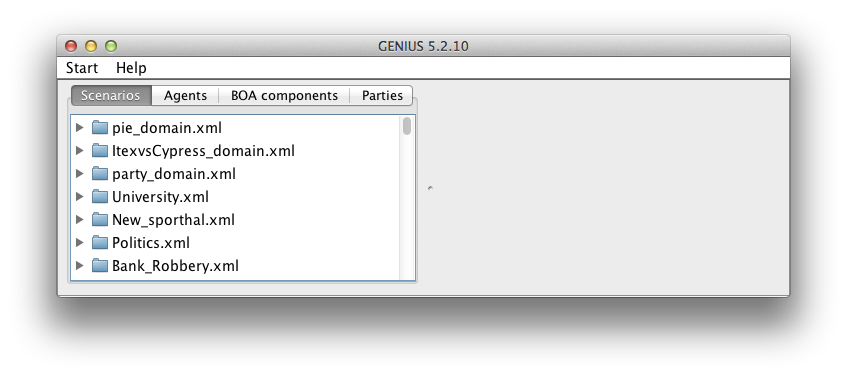
\includegraphics[width=0.6\textwidth]{media/start.png}
\caption{{\Genius} right after start-up. The left half is the components panel, the right half the status panel.}\label{Fig:negosimulator start}
\end{figure}


Progress messages and error messages are printed mainly to the standard output. On Mac OSX you can view these messages by opening the console window (double-click on Systemdisk/Applications/Utilities/Console.app). On Windows this is not directly possible. Console output can be read only if you start the application from the console window by hand, as follows. Go to the directory with the genius-XXX.jar and enter
\texttt{java -jar genius-XXX.jar}.
This will start the simulator, and all messages will appear in the console window. You may see some errors and warnings that are non-critical.

In some rare cases, parties and scenarios require more memory than allocated by default to Java. This problem can be resolved by using the Xmx and Xms parameters when launching the executable jar, for example \texttt{java -Xmx1536M -Xms1536M -jar genius-XXX.jar}. But usually, if your party runs out of memory then there is some design flaw or bug. Competitions usually are run with the default amount of java memory so it is recommended to ensure that your  party performs properly without requiring additional memory.

Please refer to chapter \ref{sec:debugging} for instructions on running {\Genius} in debug mode to debug your party.

\subsection{Running on Hi-DPI screens}
There is a bug in Java 8 that prevents windows from scaling up the {\Genius} application windows on hi-dpi screens. The bug is that Java 8 tells Windows that it will do the up-scaling itself, while java actually does not scale up anything. To fix this, do the following:

Find \verb|java.exe| and \verb|javaw.exe| that are used for running {\Genius} (Double check if you have installed multiple versions of Java). Usually they are somewhere below \verb|C:\Program Files\Java\jre\bin| or similar. For both applications, do this:

\begin{enumerate}

\item  Right click on the icon and select Properties
\item    Go to Compatibility tab
\item    Check "Override high DPI scaling behavior".
\item    Scaling performed by: set to "System" 
\end{enumerate}

%=========================================================================================
\section{Scenario Creation}\label{sec:scenariocreation}
{\Genius} offers tools to create Domains and Profiles. Currently {\Genius} supports editing the Additive and the UncertainAdditive utility space
 This section discusses how to create domains and preference profiles.


\subsection{Creating a Domain}
By right clicking on the list of available scenarios in the Domains panel a popup menu with the option to create a new domain is shown. After clicking this option a pop-up appears requesting the name for the new domain. After you enter a name and click ok, the new domain is created and a window similar to Figure~\ref{Fig:newdomain} is shown. Initially, a domain contains zero issues. We can simply add an issue by pressing the ``Add issue'' button. This results in the opening of a dialog similar to Figure~\ref{fig:createIssueD}.

\begin{figure}[htb]
	\centering
	\includegraphics[width=0.9\textwidth]{media/exampledomain.png}
\caption{{\Genius} after creating a new Example domain.}\label{Fig:newdomain}
\end{figure}

The current version of {\Genius}~supports the creation of discrete and integer issues. Starting with a discrete issue, the values of the issue should be specified. In Figure~\ref{fig:createIssueD} we show the values of the issue ``Harddisk''. Note the empty evaluation values window, later on when creating a preference profile we will use this tab to specify the preference of each value.

Instead of a discrete issue, we can also add an integer issue as shown in Figure~\ref{fig:createIssueI}. For an integer issue we first need to specify the lowest possible value and the highest value, for example the price range for a second hand car may be $[500, 700]$. Next, when creating a preference profile we need to specify the utility of the lowest possible value (500) and the highest value (700). During the negotiation we can offer any value for the issue within the specified range.

The next step is to press ``Ok'' to add the issue. Generally, a domain consists of multiple issues. We can simply add the other issues by repeating the process above. If you are satisfied with the domain, you can save it by pressing  ``Save changes''.

Finally, note that the issues of a domain can only be edited if the scenario does not (yet) specify preference profiles. This is to avoid inconsistencies between the preference profiles and the domains. 

\begin{figure}[ht]
\center
\begin{minipage}[b]{0.35\linewidth}
	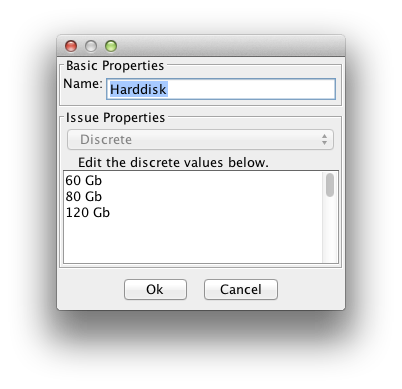
\includegraphics[width=0.95\textwidth]{media/image7a.png}
\caption{Creating a discrete issue.}
\label{fig:createIssueD}
\end{minipage}
\begin{minipage}[b]{0.55\linewidth}
	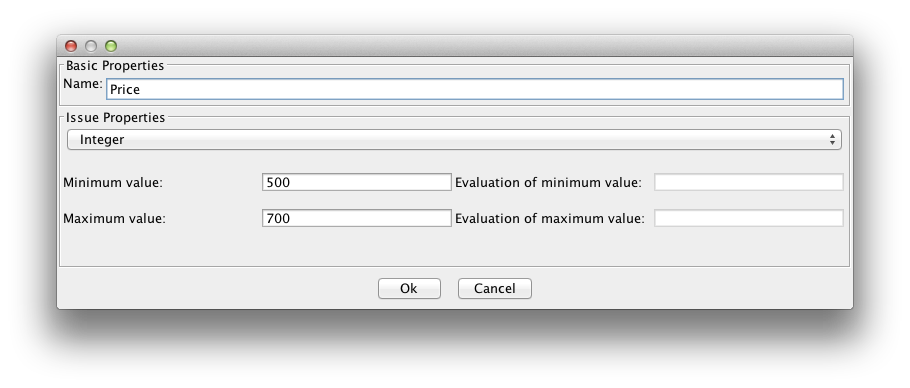
\includegraphics[width=1.0\textwidth]{media/image7b.png}
\caption{Creating an integer issue.}\label{fig:createIssueI}
\end{minipage}
\end{figure}

\FloatBarrier

\subsection{Creating an AdditiveUtilitySpace}\label{sec:createAdditive} 
Now that we created a domain, the next step is to add a set of preference profiles. Make sure that your domain is correct before proceeding, as \textit{the domain can not be changed when it contains profiles}. By right clicking on the domain a popup menu is opened which has an option to create a new preference profile. Selecting this option results in the opening of a new window which looks similar to Figure~\ref{fig:utilcreated}.

\begin{figure}[htb]
	\centering
	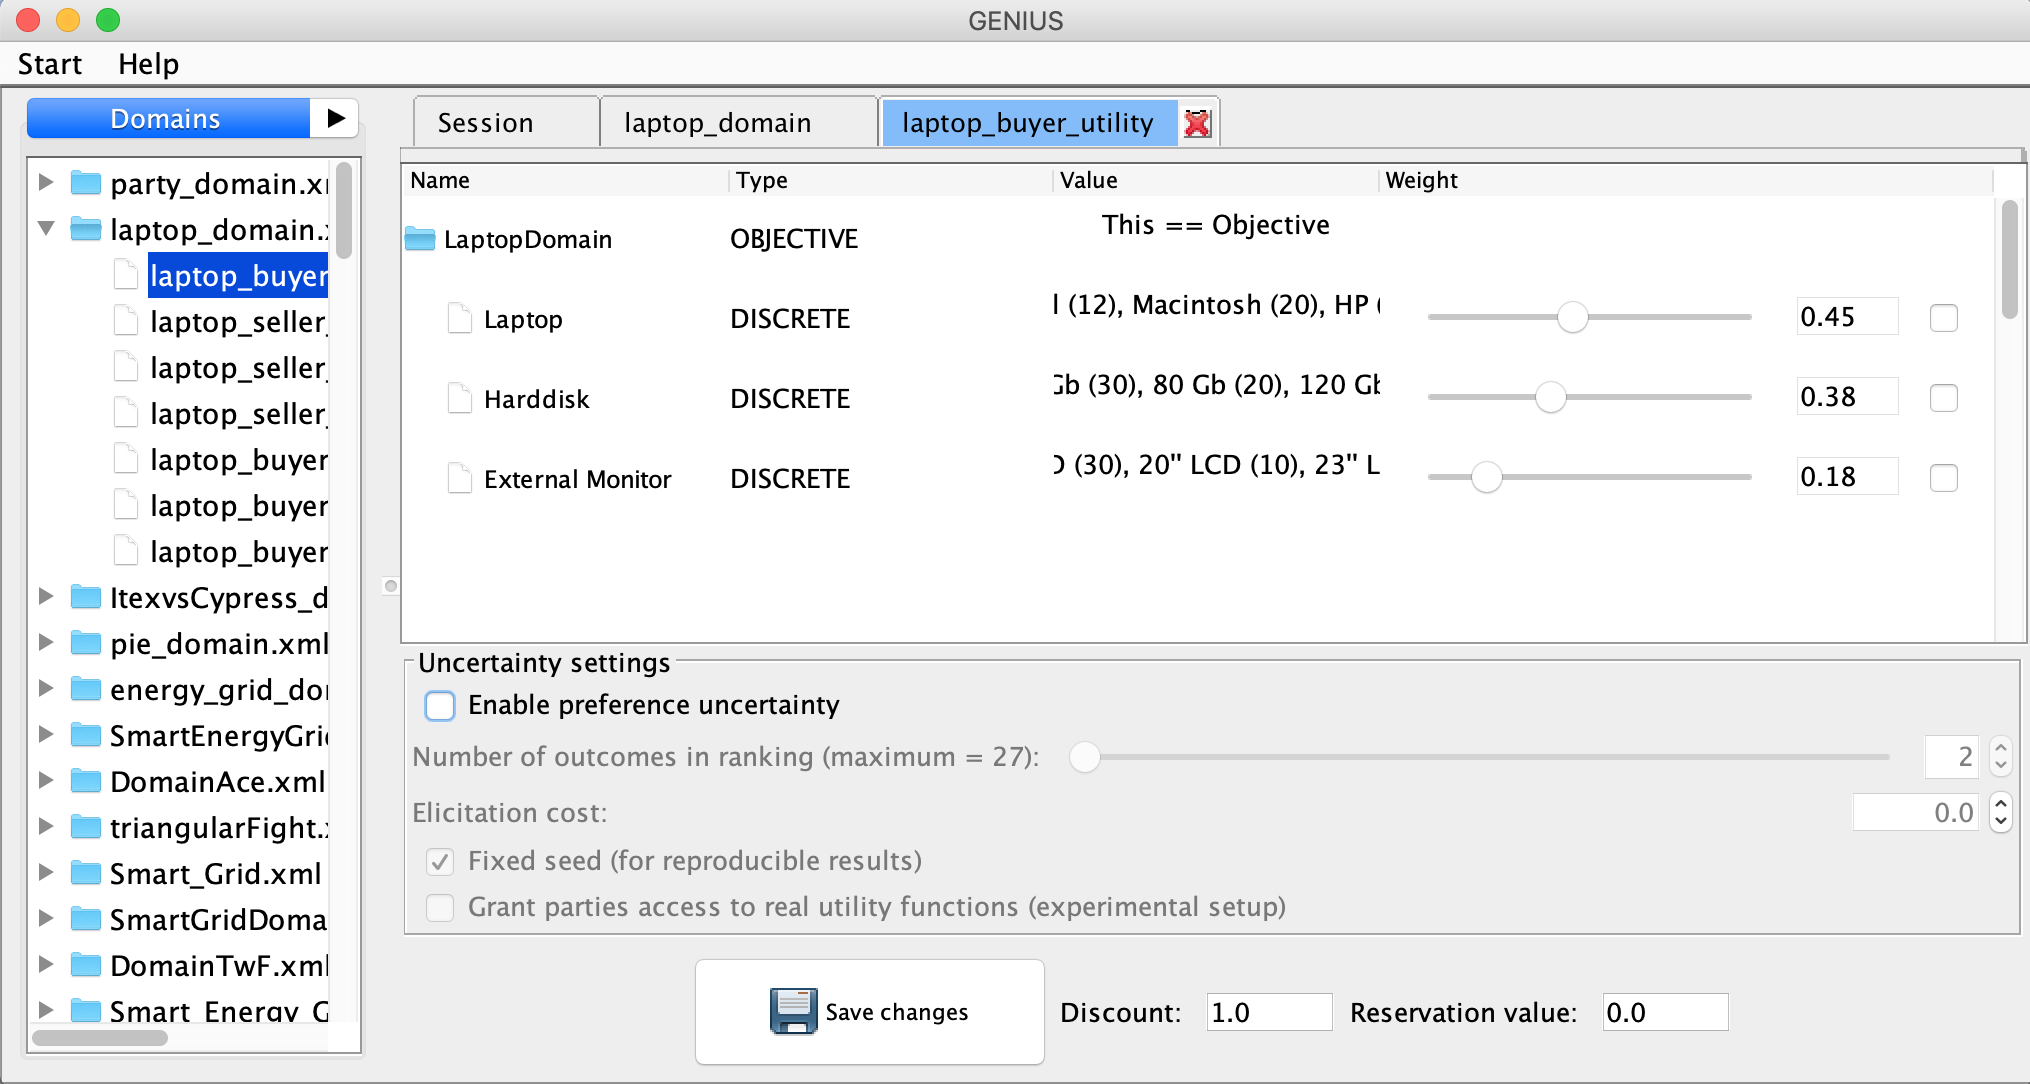
\includegraphics[width=0.8\textwidth]{media/laptop.png}
\caption{{\Genius} after creating a new utility space.}\label{fig:utilcreated}
\end{figure}

Now you are ready to start customizing the preference profile. There are three steps: setting the importance of the issues, determining the preference of the values of the issues, and configuring the reservation value and discount. Make sure that you leave the "Enable preference uncertainty" checkbox unchecked.

\begin{enumerate}
\item Adjust the relative weights of the issues by using the sliders next to that issue. Note that when you move a slider, the weights of the other sliders are automatically updated such that the all weights still sum up to one. If you do not want that the weight of another issue automatically changes, you can lock its weight by selecting the checkbox behind it. Now that we set the weights of the issues, it is a good idea to save the utility space.
\item set the evaluation of the issues. To specify the evaluation of an issue you can double click it to open a new window looking similar to Figure~\ref{fig:createIssueD} or Figure~\ref{fig:createIssueI} depending on the type of the issue.

For a discrete issue we need to specify the evaluation value of each discrete value. A specific value can be assigned any positive non-zero integer as evaluation value. During the negotiation the utility of a value is determined by dividing the value by the highest value for that particular issue. To illustrate, if we give 60 Gb evaluation 5, 80 Gb evaluation 8, and 120 Gb evaluation 10; then the utilities of these values are respectively 0.5, 0.8, and 1.0.

Specifying the preference of a integer issue is even easier. In this case we simply need to specify the utility of the lowest possible value and the highest possible value. The utility of a value in this range is calculated during the negotiation by using linear interpolation of the utilities of both given utilities.

\item The final step is to set the reservation value and discount of a preference profile. 

\item If you are satisfied with the profile you can save it by pressing ``Save changes''. 
\end{enumerate}

\subsection{Creating an UncertainAdditiveUtilitySpace and a User}

To create an uncertain additive utility space, first open or create an AdditiveUtilitySpace (section \ref{sec:createAdditive}), which defines a utility function $U$ over all possible outcomes. Check the "Enable preference uncertainty" checkbox  (Figure \ref{fig:utilcreated}) to create a UncertainAdditiveUtilitySpace. 

The resulting UncertainAdditiveUtilitySpace is a partial ordering generated from the AdditiveUtilitySpace $U$. To be precise, it is a ranking $\mathcal{O}$ of $d$ different bids in the outcome space, consistent with $U$~\cite{Tsi18}:

\begin{equation} 
\mathcal{O}=\left\{o^{(1)},o^{(2)}, \dots, o^{(d)} \right\}, \textrm{where } U(o^{(1)}) \leq U(o^{(2)}) \cdots \leq U(o^{(d)}).
\end{equation}


Use ``Nr. of outcomes in ranking'' to set $d$. The smaller you choose $d$, the higher the level of preference uncertainty. The minimal and maximal bid in the domain are always present in the ranking, which is why the smallest $d$ that can be chosen is 2. If you want to have the bid comparisons list to be a `controlled random' sequence that generates the same random ranking at every run, leave the fixed seed option enabled. If you want to generate different random bids at every run, disable the fixed seed option. If your profile is for testing purposes, also check ``Grant parties access to real utility functions''. The details of these settings are explained in section \ref{sec:partialordering}. 

The creation of an uncertain additive utility space automatically creates a User that has the ability to reveal information about the true utility of the bids against an elicitation cost in the range $[0,1]$. Use ``Elicitation cost" to set the cost of eliciting information from the User. Press "Save changes" to store your profile.

%=========================================================================================
\section{Running Negotiations}
This section discusses how to run a negotiation. There are two modes to run a negotiation:

\begin{itemize}
	\item \textbf{Session}. A single negotiation session in which a number of parties negotiate.
	\item \textbf{Tournament}. A tournament of multiparty sessions.
\end{itemize}

you start one of these by selecting them from the Start menu (Figure \ref{Fig:negosimulator start}).

Before going into detail on how each of these modes work, we first discuss the two types of parties that can be used: automated parties and non-automated parties. Automated parties are parties that can compete against other parties in a negotiation without relying on input by a user. In general, these parties are able to make a large amount of bids in a limited amount of time.

In contrast, non-automated parties are parties that are fully controlled by the user. These types of parties ask the user each round which action they should make. {\Genius}~by default includes the UIAgent -- which has a simple user interface -- and the more extensive Extended UIAgent.


\subsection{Running a Session}\label{sec:singlesessionrun}
To run a negotiation session select the menu ``Start'' and then ``Session''. This opens a window similar to Figure~\ref{Fig:multipartysession}. 

\begin{figure}[h!]
	\centering
	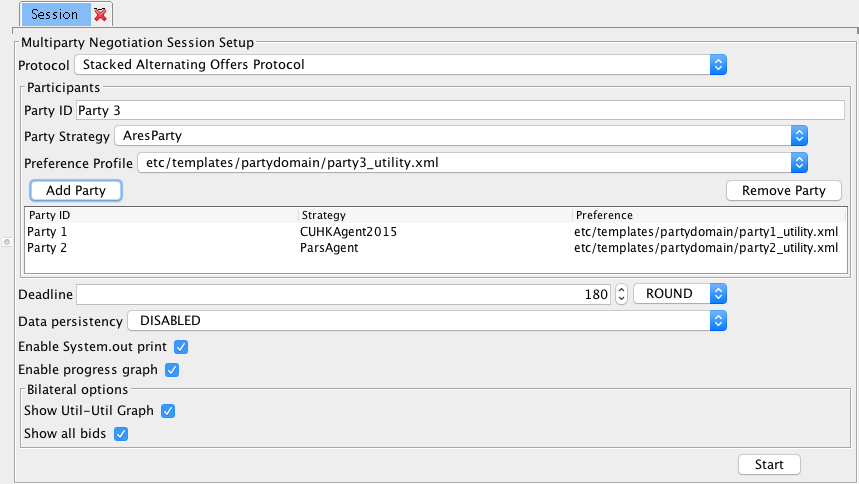
\includegraphics[width=0.5\textwidth]{media/multipartysession.png}
\caption{A multi-party negotiation session.}\label{Fig:multipartysession}
\end{figure}

The following parameters need to be specified to run a negotiation:

\medskip
\begin{minipage}{.8 \textwidth}
\begin{itemize}
	\item \textbf{Negotiation protocol}. The set of available protocols. See Chapter \ref{sec:protocols}.
	\item \textbf{Mediator}. The mediator ID and strategy that is to be used for this session. This is only visible if the protocol uses a mediator.
	\item \textbf{Participant Information}. The information (ID, strategy, profile) for the a party in the session. This information is copied into the table of participants when you click "Add Party".
	\item \textbf{A table with participants}. This table shows all currently added participants. You can add a party by setting the participant information above, and then clicking "Add Party". You can remove a party by selecting the party to remove in the table, and then clicking "Remove Party". 
	\item \textbf{Deadline}. The deadline to use. Can be "Round" or "Time". This determines the maximum duration of the session.
	\item \textbf{Data Persistency}. What kind of persistent data is available to the parties. The options are discussed in section \ref{sec:sessiongeneration}.
	\item \textbf{Enable System.out print}. If disabled, all system.out.print is suppressed during the negotiation. This is useful if for instance parties are flooding the output console, slowing down the system.
		\item \textbf{Enable progress graph}. If enabled (default), a progress chart is shown during the negotiation. You can disable this e.g. if the drawing is slowing down the system.
\item \textbf{Bilateral options} These appear only if you have exactly 2 parties added. The sub-options of this panel are
	\begin{itemize}
	\item \textbf{Show Util-Util Graph}. If enabled, the progress panel will show a graph where the utilities of the 2 parties are set along the X and Y axes. Also, the pareto frontier and nash point are shown in this graph. If disabled, it will show the default: a graph where the utilities of all parties are along the Y axis, and the time along the X axis. 
	\item \textbf{Show all bids}.  If enabled, and if 'Show Util-Util Graph' is enabled, this will show all the possible bids in the Util-Util graph.
	\end{itemize}

\end{itemize}
\end{minipage}
\medskip


The negotiation is started when you press the start button. The tab contents will change to  a progress overview panel
showing you the results of the negotiation (Figure \ref{fig:biprogress} and Figure \ref{fig:multiprogress}). The results are also stored in a log file.
 These results can be easily analyzed by importing them into spreadsheet software such as Excel.

	\begin{figure}[ht]
		\center
		\begin{minipage}[b]{0.4\linewidth}
			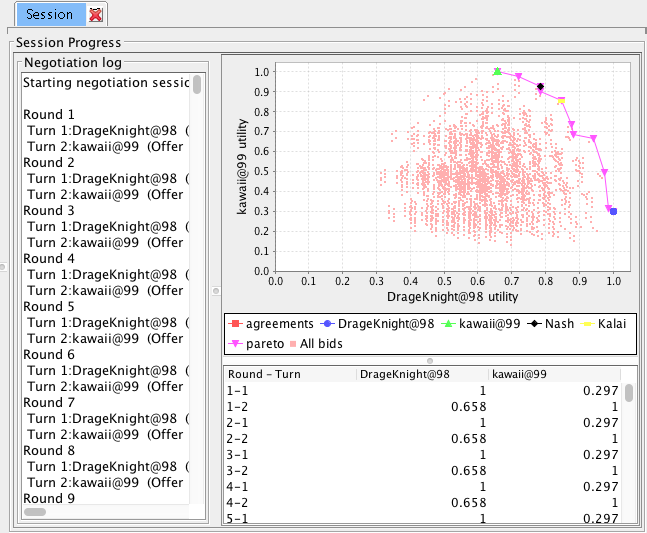
\includegraphics[width=0.95\textwidth]{media/bilateralprogress.png}
		\caption{Bilateral progress panel.}
		\label{fig:biprogress}
		\end{minipage}
		\begin{minipage}[b]{0.4\linewidth}
			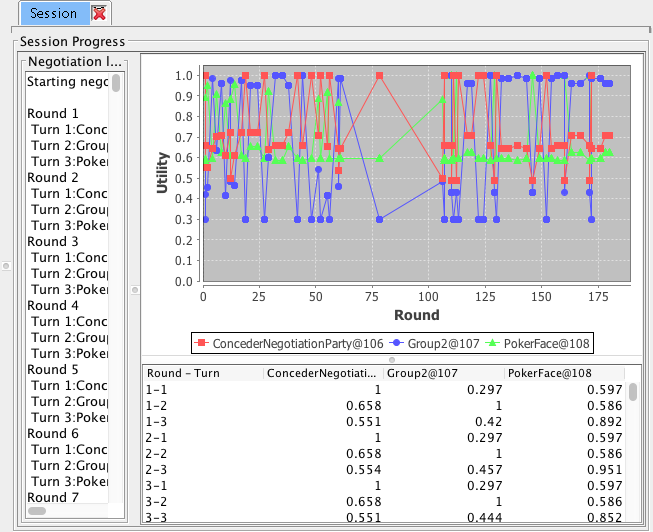
\includegraphics[width=0.95\textwidth]{media/multilateralprogress.png}
		\caption{Multilateral progress.}\label{fig:multiprogress}
		\end{minipage}
		\end{figure}
		

\subsection{Running a Tournament}
A  tournament is a set of sessions. To prepare a tournament, select  ``Start'' and then ``Tournament''. 

\begin{figure}[htb]
	\centering
	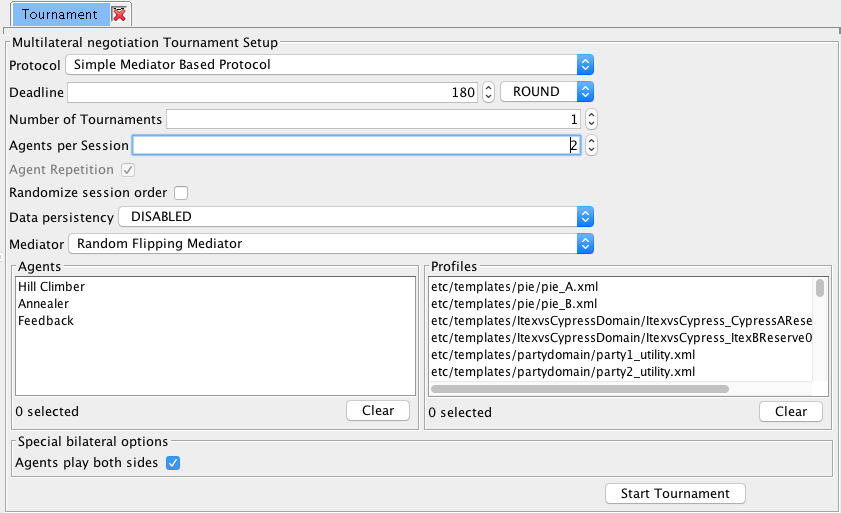
\includegraphics[width=0.7\textwidth]{media/multipartytournament.png}
\caption{Tournament}\label{Fig:multipartytournament}
\end{figure}

The Tournament tab will appear similar to Figure~\ref{Fig:multipartytournament}. This panel shows a set of tournament options. The detailed meaning of all these settings is explained in \ref{sec:sessiongeneration}.

\begin{itemize}
	\item \textbf{Protocol}. The protocol to use for each session.
	\item \textbf{Deadline}. The limits on time and number of rounds for each session.
	\item \textbf{Number of tournaments}. The number of times the entire tournament will be run.
	\item \textbf{Agents per Session}. The number of agents N to use for each session.
	\item \textbf{Agent Repetition}. whether to draw parties with or without return.
	\item \textbf{Randomize session order}. whether to randomize the session order
	\item \textbf{Data persistency}. The type of persistent data available to the parties. Same options as in section \ref{sec:singlesessionrun}.
	\item \textbf{Mediator}. The mediator to use. This option is visible only if the selected protocol needs a mediator. 
	\item \textbf{Agents}. The pool of agents to draw from. Click or drag in the agents area to (de)select agents. Click "Clear" to clear the pool.
	\item \textbf{Profiles}. The profiles pool. Click or drag in the profiles area to (de)select agents. Click "Clear" to clear the pool.
	\item \textbf{Special bilateral options}. These options appear only if Agents per session is set to 2 and is discussed in below .
\end{itemize}



\subsubsection{Bilateral special options}
If you have set 'Agents per session' to 2, and deselect 'Agent play both sides', you get an additional panel where you can select different Agents and Profiles for the B side of the 2-sided negotiation as in Figure~\ref{Fig:multipartytournament2}. 

\begin{figure}[htb]
	\centering
	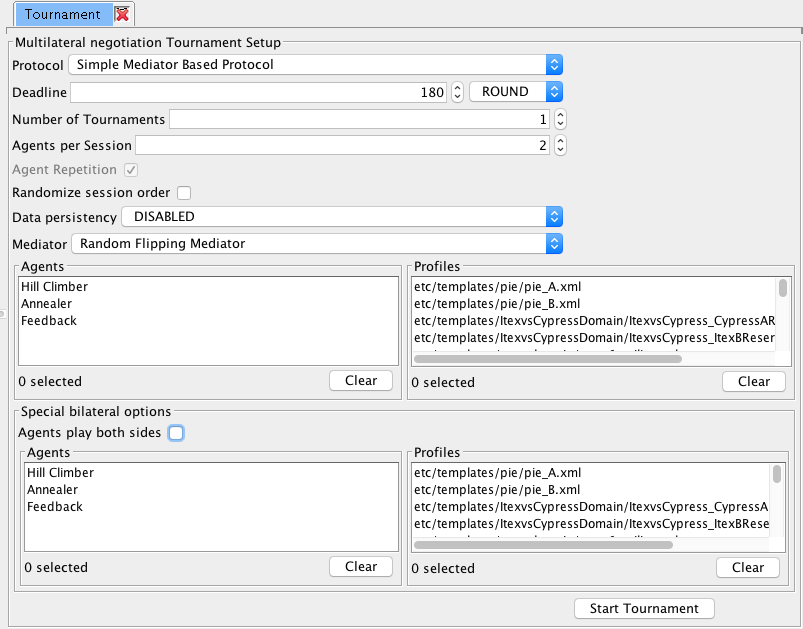
\includegraphics[width=0.7\textwidth]{media/multipartytournament2.png}
\caption{Bilateral Tournament}\label{Fig:multipartytournament2}
\end{figure}

After you click "Start Tournament", the tournament starts. The panel then is swapped for a tournament progress panel (Figure \ref{Fig:tournamentprogress}). 
In the top there is a progress bar showing the total number of sessions and the current session. The table shows all session results. The table is also saved to a $.csv$ log file in the log directory.

\begin{figure}[htb]
	\centering
	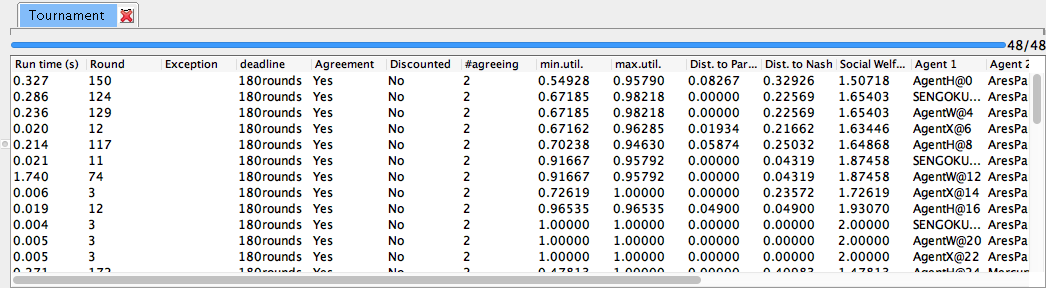
\includegraphics[width=0.9\textwidth]{media/tournamentprogress.png}
\caption{Tournament Progress panel}\label{Fig:tournamentprogress}
\end{figure}

The results of the tournament are shown on screen and also stored in a log file.  These results can be easily analyzed by importing them into spreadsheet software such as Excel.


\subsection{Running from the command line}
You can run a multi-party tournament from the command line, as follows.

\begin{enumerate}
\item Prepare an xml file that describes the settings for the tournament
\item Run the command runner and give it the prepared file 
\end{enumerate}

\subsubsection{Prepare the XML settings file}
The first step is to create an xml file containing the values needed for session generation (Section \ref{sec:sessiongeneration}).
Make a copy of the \verb|multilateraltournament.xml| file inside your genius directory and edit it (with a plain text editor).  Inside the \verb|<tournaments>| element you will find a number of \verb|<tournament>| elements. Each of these \verb|<tournament>| elements defines a complete tournament so you can run multiple tournaments using one xml file.

The contents of each \verb|<tournament>| element is as follows. The meaning of the fields is detailed in section \ref{sec:sessiongeneration}.

\begin{itemize}
\item \textbf{protocolItem}. Contains the protocol to use, in the form of a protocolItem.
\item \textbf{deadline}.  the Deadline value.
\item \textbf{repeats}. the repeats value. 
\item \textbf{persistentDataType}. The type of the persistent data.
\item \textbf{numberOfPartiesPerSession}. the Parties per session value.
\item  \textbf{repetitionAllowed}. the value for the Party Repetition. 
\item  \textbf{enablePrint}. allow agents to print. 
\item \textbf{partyRepItems}. This element contains a number of \verb|<item>| elements. Each of these party items contains a description of a party as discussed below.
\item \textbf{mediator}. the mediator, if needed. This is similar in contents to a party item discussed below. 
 \item \textbf{partyProfileItems}. This element contains a number of items. There must be at least as much as numberOfNonMediatorsPerSession. 
 \end{itemize}

We have a number of items:
\begin{itemize}

\item A profile item : contains 
	 \begin{itemize}
	\item \textbf{url} that contains the description of that party profile. These URIs point to files and therefore are of the form \verb|file:path/to/file.xml|
  	\end{itemize}

\item A party item  (and mediator) contains:
  \begin{itemize}
    \item \textbf{classPath} the java.party.class.path to the main class. That class must implement the NegotiationParty interface
    \item \textbf{properties} can contain a number of \verb|<property>| nodes with these values
    		\begin{itemize}
		\item isMediator: this property indicates the party item is a mediator. If not set, the party will be 
		run as a normal party instead of a mediator, which will probably cause protocol violations
		\end{itemize}
  \end{itemize}

\item protocol item. This item contains the protocol information: 
	\begin{itemize}
	\item \textbf{hasMediator} which is true iff protocol requires mediator
	\item \textbf{description} a one-line textual description of the mediator
	\item \textbf{classPath} the java full.class.path of the protocol class
	\item \textbf{protocolName} a brief protocol name 
	\end{itemize}
\end{itemize}



The tournament will consist of sessions created creating all permutations of \verb|<numberOfNonMediatorsPerSession>| from the partyRepItems (with or without reuse, depending on \textbf{repetitionAllowed}. The randomization also is applied to the profile items.


\subsubsection{Run the tournament}
To run the tournament, open a terminal/console and change the working directory to the genius directory.
Then enter this command (where yourfile.xml is the name of the file you just edited and XXX the version of genius that you use):

\vspace{0.5cm}
\verb|java -cp genius-XXX-jar-with-dependencies.jar genius.cli.Runner yourfile.xml|
\vspace{0.5cm}

Press return if the app prompts you for the log file location to log to  the default \verb|logs/...csv| file.

\subsection{Tournament Session Generation}\label{sec:sessiongeneration}
Instead of manually setting all the setting, a tournament generates the exact session settings from the tournament settings. These
settings are specified either in the user interface settings, or in an XML file. The parameters are:

\begin{itemize}
\item \textbf{Protocol} The protocol value is used for all sessions. See section \ref{sec:protocols}.
\item \textbf{Mediator} The mediator to use for all sessions (ignored if the protocol does not need a mediator)
\item \textbf{Deadline} The deadline is used for all sessions.  A deadline contains two values:
     \begin{itemize}
        \item \textbf{value}. This is the maximum value determining the deadline. Must be an integer $\ge 1$.
        \item \textbf{type.} Can be either $ROUND$ or $TIME$. If $ROUND$, the value is the number of rounds. If $TIME$, value is a time in seconds.
      \end{itemize}
\item \textbf{Data persistency}. The type of persistent data available to the parties. The next time a party of the same class and same profile runs in a tournament, it will receive the previously stored data. The options are 
	\begin{itemize}
	\item \textbf{Disabled}. Parties do not receive any persistent data. This is the default.
	\item \textbf{Serializable}. Parties can save anything serializable in the $PersistentDataContainer$.
	\item \textbf{Standard}. Parties receive a prepared, read only StandardInfo object inside the $PersistentDataContainer$.. 
	\end{itemize}
\item \textbf{repeats} This is also called 'number of tournaments' and determines the number of times a complete tournament will be run.
\item \textbf{Randomize Session Order} Whether all generated sessions within a tournament must be randomized.
\item \textbf{Parties per session} The number of parties to draw for each session. This excludes a possible mediator.
\item \textbf{Party Repetition} true if parties are to be drawn from the parties pool with return, false if they are to be drawn without return.
\item \textbf{Parties and Profile pool for side A}  A list from which parties and profiles will be drawn
\item \textbf{Parties and Profile pool for side B} Another list of parties and profiles. Only used with bilateral generation (see below).
\end{itemize}

The tournament generation works as follows. 

If there are exactly 2 parties per session and the parties and profiles for side B have been set, then bilateral generation is used. Otherwise, multilateral generation is used. This generation method creates an ordered list of sessions for 1 tournament.  If the 'Randomize Session Order' is set, the list is randomized. All sessions use the same protocol, mediator, deadline and data persistency.
This generation is called repeatedly, as set in 'repeats', and all generated session lists are accumulated in a big session list. This is the final result of the  tournament generation.

\subsubsection{Multilateral generation}
In multilateral generation,  all possible combinations of parties and profiles (using pool A) are generated as follows. the indicated number of parties per session $N$ are drawn from party pool A, with our without return as specified in 'Party Repetition'. Also, $N$ profile items are drawn, ordered without return, from the profiles pool. These two lists are then paired into groups of $N$ party-profile pairs. 

\subsubsection{Bilateral generation}
In bilateral generation, first a set of participants P of all combinations of 1 party and 1 profile are drawn from the side A pool. Similarly a set of participants Q is drawn for the B pool. Then, the sessions set consists of all combinations of one participant from P and another participant from Q . 





%=========================================================================================
\section{Quality Measures}\label{sec:qm}

Genius logs a large number of quality measures to log files~\cite{Baarslag12AI,Baarslag13AIT}. Logs are written both  in \verb|.csv| and \verb|.xml| format.
Logs are written to the \verb|log/| directory. Filenames contain the date and time the session/tournament started. 

The output of the log files differs, depending on whether you ran a tournament or a single session. The following subsections discuss the output for these.

Party names are printed as follows. If the party is a normal NegotiationParty, then the party will print out as something like \verb|Atlas32016@2|. The part before the '@' is the party's name, the part after the '@' is added by the runner to make the name unique. If the party is a BOA party, the name is "boa-" followed by the concatenation of its offering strategy, acceptance condition, opponentmodel and omstrategy. For example you may get this as boa party name:

\begin{verbatim}
boa-genkus.core.boaframework.offeringstrategy.anac2012.CUHKAgent_Offering-
genius.core.boaframework.acceptanceconditions.anac2012.AC_CUHKAgent-
genius.core.boaframework.opponentmodel.CUHKFrequencyModelV2-
genius.core.boaframework.omstrategy.TheFawkes_OMS@3
\end{verbatim}


\subsection{Session logs}
Both the XML and CSV log files from a session get the filename \verb|Log-Session_| followed by day and time. The contents however differ.

\subsubsection{Session CSV file}
 The \verb|.csv| file contains one line for each turn, like this:
\verb|1,1,0.0055248618784530384,AgentHP2_main@0,(Offer  bid:Bid[Food: Chips and Nuts, ...ials, ])|

The columns are, in order:
\begin{enumerate}
\item round number.
\item turn number
\item the time of agreement, in the range [0,1] where 0 means the start of the session and 1 the maximum time/number of rounds allowed for the negotiation. 
\item the party that acted.
\item the action that the party did. The action consists of the action type name ("Offer", "Accept", "EndNegotiation", etc) and the bid details if available.
\end{enumerate}


\subsubsection{Session XML file}
When running a session, the XML file contains only the details of the final outcome of the negotiation.

The fields in the \verb|NegotiationOutcome| element:\label{table:NegotiationOutcome}
\begin{enumerate}
\item currentTime: the moment when the final outcome was available. 
\item timeOfAgreement, agreement time in the range [0,1] where 0 means the start of the session and 1 the maximum time/number of rounds allowed for the negotiation. 
\item lastAction: the last action that was done
\item the domain that was being run
\item bids: the total number of bids that have been done in this session
\item the total run time in seconds
\item the outcome : the final accepted bid , or "-" if there was no final agreement
\item the startingAgent,
\item the deadline = maximum amount of time/rounds for this session.
\end{enumerate}

and then, for each of the parties that participated a "resultsOfAgent" element containing:
\begin{enumerate}
\item the party's name. 
\item the party's description.
\item the party's utilityspace filename.
\item the full party class path.
\item the user utility (the true performance of the agent: equal to the discounted final utility minus the total user bother)
\item the final utility (un-discounted) of this party, or 0 if there was no agreement.
\item the final utility (discounted).
\item the value of discount(1,1). This is the remaining utility that a un-discounted utility of 1 would have at the end time (t=1). For default discount formulas, this equals the 'discount factor'.
\item the total user bother. This quantifies how much the agent elicited the User in the uncertainty setting. Equal to 0 if the agent did not elicit anything or the negotiation did not take place under uncertainty.
\end{enumerate}


Here's an example
\begin{verbatim}
<?xml version="1.0"?>
<Session>
       <NegotiationOutcome currentTime="Mon Oct 14 11:51:49 CEST 2019" 
         timeOfAgreement="0.09836065573770492" 
         lastAction="(Accept  bid:Bid[Food: Chips and Nuts, Drinks: Handmade Cocktails, Location: Party Room, ...   	  
         domain="etc/templates/partydomain/party_domain.xml" bids="10" runtime="0.023675353" finalOutcome="Bid[...
         startingAgent="-" deadline="60rounds">
              <resultsOfAgent agent="TOP_3_Agent" agentDesc="BOA(AC_Top3,O_S Top3,Default,Offer Best Bids)" 
                   utilspace="etc/templates/partydomain/party1_utility.xml" 
                   agentClass="genius.core.repository.boa.BoaPartyRepItem$1" 
                   userUtility="0.7398203133659815" finalUtility="0.7848203133659816" 
                   discountedUtility="0.7848203133659816" discount="1.0" totalUserBother="0.045">
              </resultsOfAgent>
              <resultsOfAgent agent="TimeDependentAgentLinear@1" agentDesc="concedes linearly with time" 
                   utilspace="etc/templates/partydomain/party2_utility.xml" 
                   agentClass="agents.TimeDependentAgentLinear" 
                   userUtility="0.9285654723948509" finalUtility="0.9285654723948509" 
                   discountedUtility="0.9285654723948509" discount="1.0" totalUserBother="0.0">
              </resultsOfAgent>
        </NegotiationOutcome>
</Session>\end{verbatim}



\subsection{Tournament logs}
All log files from a tournament get the filename \verb|tournament-| followed by day and time followed by the domain name and an extension.
There are 3 log files created: a log.csv file, a log.xml file and a logStats.xml file.

If you terminate a tournament before it completes, the .log. files will be written up to the last completed session and there will be no logStats file.

\subsubsection{Tournament log.csv file}

tournament .csv files start with these a line containing \verb|sep=;| indicating that we use the comma as separator character for fields.
Then there is a table header typically looking like this (if there are 3 parties in each session, and all this on 1 line)
\begin{verbatim}
Run time (s);Round;Exception;deadline;Agreement;Discounted;#agreeing;min.util.;max.util.;
  Dist. to Pareto;Dist. to Nash;Social Welfare;
  Agent 1;Agent 2;Agent 3;
  Utility 1;Utility 2;Utility 3;
  Disc. Util. 1;Disc. Util. 2;Disc. Util. 3;
  Perceived. Util. 1;Perceived. Util. 2;Perceived. Util. 3;
  User Bother 1;User Bother 2;User Bother 3;
  User Util. 1;User Util. 2;User Util. 3
  Profile 1;Profile 2;Profile 3
\end{verbatim}

The rest of the log file contains one line for each final session outcome, matching the columns in the header:

\begin{enumerate}
\item the run time of that session (seconds). 
\item the number of rounds that were completed
\item the exception message, if an exception occured
\item the deadline = maximum amount of time/rounds for this session.
\item whether an agreement was reached (Yes) or not (No).
\item whether there was a discount factor (i.e. discount(1,1) is not 1) (Yes or No).
\item the final number of agreeing parties 
\item the minimum utility achieved by the parties
\item the maximum utility achieved by the parties
\item the distance to the pareto curve (the nearest bidpoint on the pareto)
\item the distance to the nash optimum point
\item the distance to the social welfare point
\item the names of all parties
\item the un-discounted utilities of all parties.
\item the discounted utilities of all parties
\item the perceived utilities of all parties. 
\item the user bother of all parties
\item the user utility of all parties
\item the profile names of all the parties
\end{enumerate}

If the profile is a Utilityspace, then the discounted and un-discounted utilities are as in the original utilityspace provided to the agent. The perceived utility in that case equals to the discounted utility. The user utility as well, and the user bother is equal to 0.
If the profile is a partially ordered profile, the core (but not the agent) knows the utility in the AdditiveUtilitySpace that was used to create the profile. In that case, the un-discounded and discounted utilities are utilities as in the AdditiveUtilitySpace. The agent is provided with another AdditiveUtilitySpace that was generated based on the partially ordered profile, and usually will differ from the original AdditiveUtilitySpace. The perceived utility is the (discounted) utility of the bid in that estimated space. 
The perceived utility is available only in the CSV file in tournament logs, not in XML log files. The user bother represents how much the agent performed elicitation actions. The user utility represents the true performance of the agent, it is equal to the discounted utility minus the user bother.

For example, one line of the output can look like this (all on 1 line)

\begin{verbatim}
4.965;173;;180rounds;Yes;No;3;0.58083;0.95256;0.00000;0.44991;2.13706;
ClockworkAgent@14;Farma@15;Caduceus@16;
0.5808333333333333;0.6036696609166442;0.9525594478616071;
0.5808333333333333;0.6036696609166442;0.9525594478616071;
0.5808333333333333;0.6036696609166442;0.9525594478616071;
0.0;0.0;0.0;
0.5808333333333333;0.6036696609166442;0.9525594478616071;
party1_utility.xml;party2_utility.xml;party3_utility.xml
\end{verbatim}

\subsubsection{Tournament log.xml file}

The .log.xml file contains one \verb|<NegotiationOutcome>| element for each completed round.
These elements are formatted exactly as in \ref{table:NegotiationOutcome}.

\subsubsection{Tournament logStats.xml file}
The logStats.xml file contains for each of the parties that participated in the tournament statistical info:

\begin{enumerate}
\item agentname: the party's name (full class path)
\item totalUndiscounted: the total sum of the un-discounted utilities that it achieved
\item totalDiscounted: the total sum of the discounted utilities that it achieved
\item numberOfSessions: the total number of sessions that it participated in
\item totalNashDist: the accumulated distances to the Nash Point
\item totalWelfare: the accumulated distances to the Social Welfare Point
\item totalParetoDistance: the accumulated distances to the Pareto frontier
\item meanDiscounted: totalDiscounted /  numberOfSessions
\item meanUndiscounted: totalUndiscounted /  numberOfSessions
\item meanNashDistance: totalNashDistance /  numberOfSessions
\item meanWelfare: totalWelfare /  numberOfSessions
\item meanPareto: totalPareto /  numberOfSessions
\end{enumerate}


%
%
%\subsection{Analyzing Logs using Excel}~\label{sec:analysisExcel}
%The logs are in XML and CSV format, so we can easily analyze them with Excel. Note that the following discussion does not apply to the starter edition of Excel, as it does not support Pivot tables.
%
%The XML data of the standard log can be converted to a normal table by importing the data into Excel using the default options. This results in a large table showing the result for both agents A and B for each session. Analyzing these results manually is complicated, therefore we recommend to use pivot tables. Pivot tables allow to summarize a large set of data using statistics and can be created by selecting ``Insert'' and then ``Pivot Table''. To illustrate, by dragging the \textit{agentName} in ``Row Labels'' and the \textit{discountedUtility} in ``Values'' (see Figure~\ref{fig:pivottable}), we can easily see which agent scored best in the tournament. If solely the amount of matches of each agent is displayed, you need to set the ``Value Field Settings'' of \textit{discountedUtility} to average instead of count.
%
%\begin{figure}[htb]
%	\centering
%	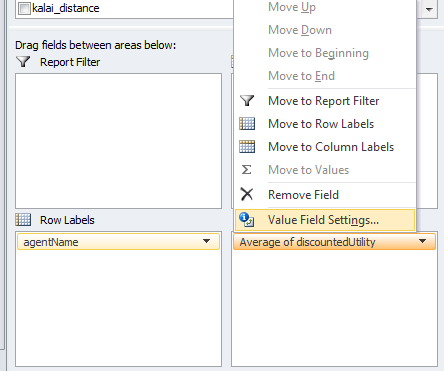
\includegraphics[width=0.4\textwidth]{media/PivotTable.png}
%\caption{Configuration required to summarize the discounted utility of each agent.}\label{fig:pivottable}
%\end{figure}


%=========================================================================================

\section{Creating a Negotiation Party}\label{sec:createagent}
To create an negotiation party, we suggest to follow the instructions in the Appendix (Section \ref{sec:appendix}) and start with one of the examples.
You can then proceed by changing the example.


\subsection{Example Parties}
The {\Genius} zip file contains a number of example parties: the bilateral examples, multiparty example, and the storage example. To compile an example, set up your workspace as in the appendix (Section \ref{sec:appendix}) and copy an example folder into  \verb|src/|.

\begin{enumerate}
	
\item The bilateral examples illustrate how to develop agents for bilateral negotiations. They illustrate the use of the domain, preferences, offers, the BOA framework, and preference uncertainty:
\begin{itemize}
	\item  The \textit{RandomBidderExample} is the easiest example to start with. This simple example agent makes random bids above a minimum target utility and demonstrates the core uses of offers and utility.
	\item  The \textit{BoaPartyExample} shows how to create an independent agent out of several BOA components and how to handle preference uncertainty.
	\item  The \textit{CustomUtilitySpacePartyExample} shows how a party can deal with preference uncertainty by defining a custom \textit{UtilitySpace} based on the closest known bid.
\end{itemize}

You can run all these agents with an UncertainAdditiveutilitySpace (for example the profiles with preference uncertainty defined on the \verb|party_domain.xml|, namely: \verb|party1_utility_u|$N$\verb|.xml| and \verb|party2_utility_u|$N$\verb|.xml|).
	
\item The multiparty example just accepts any acceptable bid with a random probability of 0.5.

\item The storage example demonstrates using the persistent data storage. This example is showing how the storage can be used to wait a little longer every next time the party is in a negotiation.

To run this example, you need to set up {\Genius} to allow persistent data storage (the default is off). In the {\Genius} tournament setup panel, use the following settings
\begin{itemize}
\item  number of tournaments= 20
\item  agents per session =2
\item  persistency=standard
\item  agent side A: GroupX, \verb|party1_utility.xml|
\item  agent side B: Random Party, \verb|party6_utility.xml|
\end{itemize}

and start the tournament and check the number of rounds till agreement: it will increase every session.

Now run another tournament with the same settings but pick select both \verb|party1_utility.xml| and \verb|party2_utility.xml|. Run the tournament.
Now you will see that the the number of rounds till agreement goes up every other run. This is because your party gets a different profile every other run and thus there are persistent data stores, one for each profile. 



\end{enumerate}

\subsection{Implementing NegotiationParty}
This section discusses details of implementing a NegotiationParty.  

Every party must at least implement the \texttt{genius.core.parties.NegotiationParty} interface (Table \ref{table:NegotiationPartyInterface}),  Also the implementation must have a public default (no-argument) constructor. Please refer to the javadocs for details on the parameters.

\begin{table*}[t]
  \centering
  \begin{tabular}{|p{4cm}|p{7cm}|}
  \hline
  Method & description \\
  \hline\hline
    init &Initializes the party, informing it of many negotiation details. This is be called exactly once by the negotiation system, immediately after construction of the class  \\
    chooseAction & When this function is called, it is expected that the Party chooses one  of the actions from the possible action list and returns an instance of the chosen action. \\
    receiveMessage & This method is called to inform the party that another NegotiationParty chose an Action.\\
    getDescription & Returns a human-readable description for this party \\
    getProtocol & The actual supported MultilateralProtocol. Usually this returns StackedAlternating\-Offers\-Protocol. Your party should override this if it supports a another protocol\\
    negotiationEnded & This is called to inform the party that the negotiation has been ended. This allows the party to record some final conclusions about the run\\
    \hline
  \end{tabular}
  \caption{Methods of NegotiationParty. Check the javadoc for all the details}
  \label{table:NegotiationPartyInterface}
\end{table*}


For convenience, we recommend you extend the class \texttt{genius.core.parties.AbstractNegotiationParty} which is a basic implementation of NegotiationParty. This class also provides convenient support functions for building your party.

Your party might need to check the exact type of the provided AbstractUtilitySpace (inside NegotiationInfo), for instance if your party supports for example only AdditiveutilitySpace. Also check the provided UserModel, if that is set (not null) then this overrides the value returned by getUtilitySpace..

A number of useful classes is given in \ref{tab:agentclass}. The javadoc contains the full details of all available classes. We recommend to use the javadoc included with the distribution to check the details of all the involved classes.  Notice that some classes, e.g. SortedOutcomeSpace, may take a long time and large amounts of memory to sort a large bid space, which may exceed the available time and space for your party. Therefore these methods should be used with caution.

\begin{table}
\begin{tabular}{m{0.9\textwidth}}
\hline
\texttt{NegotiationInfo}\\
The context of the negotiation: the partial profile ("UserModel"), utility space, the timeline and deadline, the agentID and persistent data container.\\
\hline
\texttt{UtilitySpace}\\
The preference profile of the scenario allocated to the party. It is recommended to use this class when implementing a model of the opponent's preference profile.\\
\hline
\texttt{Timeline }\\
Use timeline for every time-related by using \texttt{getTime()}.\\
\texttt{Action chooseAction(List<Class<? extends Action>> possibleActions)}\\
This function should return the action your party wants to make next.\\
\hline
\texttt{Action}\\
Superclass of negotiation actions like Offer, Accept and EndNegotiation..\\
\hline
\texttt{BidHistory}\\
a structure to keep track of the bids presented by the party and the opponent.\\
\hline
\texttt{SortedOutcomeSpace}\\
a structure which stores all possible bids and their utilities by using BidIterator. In addition, it implements search algorithms that can be used to search the space of possible bids for bids near a given utility or within a given utility range. WARNING (1) SortedOutcomeSpace iterates over all bids and thus might be unusable in large bidspaces (2) Some parties have created their own copy of SortedOutcomeSpace, so be careful to pick the genius.core version. \\
\hline
\texttt{BidIterator}\\
a class used to enumerate all possible bids. Also refer to \textit{SortedOutcomeSpace}.\\
\hline
\texttt{BidDetails}\\
a structure to store a bid and its utility.\\
\hline
\end{tabular}

\caption{Important classes used for creating a NegotiationParty.}
\label{tab:agentclass}
\end{table}

\FloatBarrier

\subsubsection{Receiving the Opponent's Action}\label{sec:receiveAction}
The \texttt{ReceiveMessage(Action opponentAction)} informs you that the opponent just performed the action \texttt{opponentAction}. The \texttt{opponentAction} may be  \texttt{null} if you are the first to place a bid, or an \texttt{Offer}, \texttt{Accept} or \texttt{EndNegotiation} action.
The \texttt{chooseAction()} asks you to specify an \texttt{Action} to send to the opponent.

In the SimpleAgent code, the following code is available for \texttt{receiveMessage}. The SimpleAgent stores the opponent's action to use it when choosing an action.

\begin{lstlisting}
public void receiveMessage(Action opponentAction) {
	actionOfPartner = opponentAction;
}
\end{lstlisting}

\subsubsection{Choosing an Action}\label{sec:chooseAction}
The code block below shows the code of the method \texttt{chooseAction} for SimpleAgent. For safety, all code was wrapped in a try-catch block, because if our code would accidentally contain a bug we still want to return a good action (failure to do so is a protocol error and results in a utility of 0.0).

The sample code works as follows. If we are the first to place a bid, we place a random bid with sufficient utility (see the .java file for the details on that). Else, we determine the probability to accept the bid, depending on the utility of the offered bid and the remaining time. Finally, we randomly accept or pose a new random bid.

While this strategy works, in general it will lead to suboptimal results as it does not take the opponent into account. More advanced parties try to model the opponent's strategy or preference profile.

\begin{lstlisting}
public Action chooseAction() {
	Action action = null;
	Bid partnerBid = null;
	try {
		if (actionOfPartner == null)
			action = chooseRandomBidAction();
		if (actionOfPartner instanceof Offer) {
			partnerBid = ((Offer) actionOfPartner).getBid();
			double offeredUtilFromOpponent = getUtility(partnerBid);
			double time = timeline.getTime();
			action = chooseRandomBidAction();
			Bid myBid = ((Offer) action).getBid();
			double myOfferedUtil = getUtility(myBid);
			// accept under certain circumstances
			if (isAcceptable(offeredUtilFromOpponent, myOfferedUtil, time))
				action = new Accept(getAgentID(), partnerBid);
		}
		if (timeline.getType().equals(Timeline.Type.Time)) {
			sleep(0.005); // just for fun
		}
	} catch (Exception e) {
		 // best guess if things go wrong. Notice this may still fail
		action = new Accept(getAgentID(), partnerBid);
	}
	return action;
}
\end{lstlisting}

The method \textit{isAcceptable} implements the probabilistic acceptance function$P_\text{accept}$:

\begin{equation}
	P_\text{accept} = \dfrac{u - 2ut + 2\left(t - 1 + \sqrt{(t - 1)^2 + u(2t - 1)}\right)}{2t - 1}
\end{equation}
where $u$ is the utility of the bid made by the opponent (as measured in our utility space), and $t$ is the current time as a fraction of the total available time. Figure~\ref{Fig:Paccept} shows how this function behaves depending on the utility and remaining time. Note that this function only decides if a bid is acceptable or not. More advanced acceptance strategies (cf.~\cite{Baarslag13AAMAS,Baarslag13DSS,ANAC2010KawExt} can also take into account other factors and actions such as \texttt{EndNegotiation}.

\begin{figure}[htb]
	\centering
	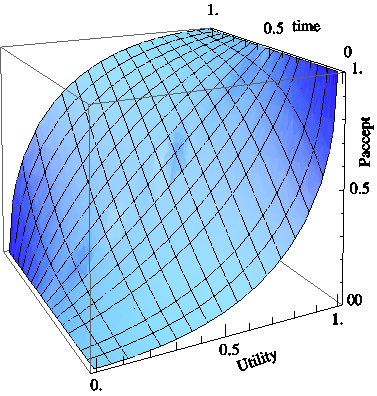
\includegraphics[width=0.3\textwidth]{media/image21.png}
	\caption{$P_\text{accept}$ value as function of the utility and time (as a fraction of the total available time).}\label{Fig:Paccept}
\end{figure}
 




\subsection{Implementing a party with preference uncertainty}
\label{sec:newUncertainAgent}

In order to program an agent with preference uncertainty, we recommend that your agent extends the \textit{AbstractNegotiationParty} class. That class has some support functions that load the normal utilityspace with an approximation that is useful for plotting outcomes. 
% This example is not yet there. 
%An example of an agent that can work with uncertainty is the \textit{UncertaintyAgentExample}. 
%When referring to code in this section, this will be code from either the \textit{AbstractNegotiationParty} class or the \textit{UncertaintyAgentExample}.

\subsubsection{Overriding functions}
In order to change the way your agent handles preference uncertainty, you can override the \textit{estimateUtilitySpace()} function. This function in AbstractNegotiationParty returns an \textit{AbstractUtilitySpace} object. In the \textit{AbstractNegotiationParty} class, this code looks as follows:
 \begin{lstlisting}
public AbstractUtilitySpace estimateUtilitySpace() {
	Domain domain = getDomain();
	AdditiveUtilitySpaceFactory factory 
	    = new AdditiveUtilitySpaceFactory(domain);
	BidRanking bidRanking = userModel.getBidRanking();
	factory.estimateUsingBidRanks(bidRanking);
	return factory.getUtilitySpace();
}
\end{lstlisting}

As can be seen from the function, a custom \textit{AbstractUtilitySpace} is created using the domain and the bid ranking. This function approximates the utility function using a simple counting heuristic. This heuristic does not perform very well, so there is need to implement your own function. An example is included in the \textit{UncertaintyAgentExample}. In this example, the \textit{AbstractNegotiationParty} class is extended and the \textit{estimateUtilitySpace()} function is overridden. Overriding this function can be done as follows:
\begin{lstlisting}
@Override
public AbstractUtilitySpace estimateUtilitySpace() 
{
	return new AdditiveUtilitySpaceFactory(
	            getDomain()).getUtilitySpace();
}
\end{lstlisting}

This function overrides the standard function and implements its own method to estimate the Utility space. Currently, this returns a utility function with equal weights and values set to zero. To estimate the utility function, you can use the \textit{BidRanking} class. The bid ranking for the current session can be accessed using \textit{userModel.getBidRanking()}. The next section will show what information is included in the \textit{BidRanking}.

\subsubsection{Bid Ranking}
When running an uncertain agent, all utility information is given through a bid ranking. This bid ranking consists of an ordering of different bids for the current domain. The ranking that the agent receives is ordered from low utility to high utility. This ranking can be used to estimate a utility function. 

The \textit{BidRanking} class consists of a list of \verb|Bid|s. To obtain the \textit{Bid} classes from the \textit{Bidranking}, you can use the \textit{getBidOrder()} function on the \textit{Bidranking} object. This object is obtained in the agent using \textit{userModel.getBidRanking()}. Check the javadoc for more details, and we suggest you check the source code of BidRanking, and makes it a little easier to compare the original utilityspace with the estimation.

To access the list of \textit{Bid} objects directly, you can use the following snippet:
\begin{lstlisting}
List<Bid> bids = userModel.getBidRanking().getBidOrder();
\end{lstlisting}

The bids that are obtained from the \textit{BidRanking} using the \textit{getBidOrder()} function are listed from low utility to high utility. This means that the first element in the list has the lowest utility score. When iterating over the list, every next bid will be either valued \textbf{higher or the same} as the current bid in the list.

\textit{BidRanking} also contains the recommended utility values through \textit{getLowUtility()} and \textit{getHighUtility()}. These values can be used for the worst and best bid in the list.


\subsubsection{Elicitation through the User}
An agent working under preference uncertainty may elicit information about the true utility to improve its user model against an elicitation cost. All elicitation actions are implemented as methods in the \textit{User} class. As of right now, the only elicitation action an agent can make is \textit{elicitRank}. \textit{elicitRank} takes as input a bid $b$ and a User Model $userModel$, and returns an updated User Model corresponding to \textit{userModel} augmented with $b$ in the Bid Ranking. To call \textit{elicitRank}, an agent must call it through the User object in this way:
\begin{lstlisting}
userModel = user.elicitRank(b, userModel);
\end{lstlisting}

\textit{elicitRank} is performed against an elicitation cost that the User holds as an attribute. To obtain the elicitation cost, an agent can use \textit{user.getElicitationCost()}. Each time \textit{elicitRank} is called by an agent, this cost is added to the total bother which is an attribute of User as well. To obtain the total bother, an agent can use \textit{user.getTotalBother()}. 
A good thing to keep in mind when using \textit{elicitRank} is that the total bother won't get incremented it you are trying to call it with a bid that is already in the User Model. 

Note: As of right now, the total bother is only implemented as constant increments of the elicitation cost. In theory however, it could be a very different function. All such possibilities are what we call bother cost functions. Future developments will explore extensions of the User class to support different types of bother cost functions.


\subsubsection{Accessing the real utility space for debugging}
If the utiltity space was saved with the ``experimental setup'' checkbox enabled (Figure \ref{fig:utilcreated}) then your agent can access the real utility function. Such a utility space can be used to verify the utility function that your agent creates itself. In order to get access to this function, the userModel should be cast to an \textit{ExperimentalUserModel} object. This can be done as follows:
\begin{lstlisting}
ExperimentalUserModel e = (ExperimentalUserModel) userModel;
UncertainAdditiveUtilitySpace realUSpace = e.getRealUtilitySpace();
\end{lstlisting}

Now, you will have access to the real utility space with \textit{realUSpace}.

\subsubsection{Preference uncertainty agent checklist}
This section will give a short overview of what to do in order to enable your agent to work with preference uncertainty. You should take the following steps:
\begin{enumerate}
    \item Extend the \textit{BoaParty} or \textit{AbstractNegotiationParty} class (examples can be found in the \textit{bilateralexamples} folder).
    \item Override the \textit{estimateUtilitySpace()} function that returns an \textit{AbstractUtilitySpace} class.
    \item Using the \textit{getDomain()} function and the \textit{BidRanking}, create an estimation for the utility function. (E.g. Counting, Machine Learning, Statistical methods, etc.; see for example:~\cite{Ayd14,BaarslagValueOfInformation,UTAGMS,Ros16,Sri73,Tsi18,Zin18})
    \item Implement the normal methods necessary for the agent to do the bidding. This is the same as for normal agents; the preference uncertainty is only used on startup of the agent in order to estimate the utility function.
\end{enumerate}


\subsection{Loading a NegotiationParty}

You need to load your custom party into the {\Genius} party repository in order to use it. After adding, your party will appear in the combo boxes in the multilateral tournament runner and session runner where you can select the party to use.

Locate the Parties repository tab in the GUI (Figure \ref{fig:partiesrepo}). Right click in this area and select "Add Party". A file browser panel pops up. Browse to  your compiled \verb|.class| file that implements the NegotiationParty and select it. Typically Eclipse compiles into \verb|bin|. Your party will appear at the bottom of the parties repository. The \verb|partyrepository.xml| file is automatically updated accordingly.

\begin{figure}[h!] 
	\center
	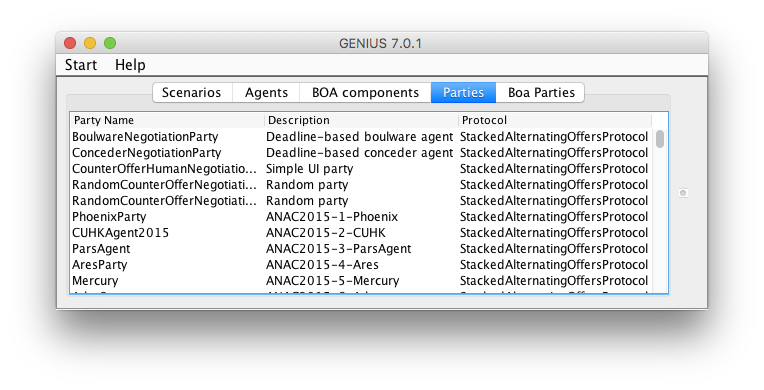
\includegraphics[width=10cm]{media/partiesrepo.png}
	\caption{The parties repository.}
	\label{fig:partiesrepo}
\end{figure}


To do this manually without using the GUI, quit {\Genius}, open the \verb|partyrepository.xml| file \footnote{This file is automatically created the first time you run {\Genius}}  and add a section like this

\begin{lstlisting}
<partyRepItem classPath="full.class.of.your.party" <properties/> />
\end{lstlisting}

After that you can restart {\Genius} so that it loads the new party.
\FloatBarrier

\subsection{Third party code}
You should not use maven or jars to add dependencies for your party. The reason is {\Genius} or other parties might already have another version of your library in use. Java 8 can not deal properly with multiple versions of the same library within a single JVM. The result would be inconsistent, incorrect or buggy behaviour, or even crashes.

Instead, if you want to use a third party library, you will have to include all the source code of that library with your code, including all sub-dependencies. Also ensure the imports in all sources are renamed accordingly. The code should be copied inside the package name of your party, instead of using the original package name of that library (so do not use "org.apache" for instance). This is to ensure that we are really running your party on the specific version of the library that your party needs and to avoid version conflicts (java will run an unspecified version of the library in case of conficts). 


%=========================================================================================
\section{Creating a BOA Party}\label{sec:boa}
Instead of implementing your negotiating party from scratch, you can create a BOA party using the \textit{BOA framework}~\cite{BaarslagBOA}.
The BOA negotiation party architecture allows to reuse existing components from other BOA parties. Many of the sophisticated party strategies that currently exist are comprised of a fixed set of modules. Generally, a distinction can be made between four different modules: one module that decides whether the opponent's bid is acceptable (\textit{acceptance strategy}); one that decides which set of bids could be proposed next (\textit{offering strategy}); one that tries to guess the opponent's preferences (\textit{opponent model}), and finally a component which specifies how the opponent model is used to select a bid for the opponent (\textit{opponent model strategy}). The overall negotiation strategy is a result of the interaction between these components.

The advantages of separating the negotiation strategy into these four components (or equivalently, fitting a party into the BOA framework) are threefold: first, it allows to \textit{study the performance of individual components}; second, it allows to \textit{systematically explore the space of possible negotiation strategies}; third, the reuse of existing components \textit{simplifies the creation of new negotiation strategies}~\cite{BaarslagComponentAnalysis}.

{\bf Warning:} Many of the provided BOA components currently assume a single opponent party, which will behave incorrectly when used with multiple opponents. We recommend checking the source code of the BOA components you want to use, or write your own components if you are creating a multilateral NegotiationParty.


\subsection{Components of the BOA Framework}
A negotiation party in the BOA framework, called a \textit{BOA party}, consists of four components:
\begin{description}
  \item[Offering strategy] An offering strategy is a mapping which maps a negotiation trace to a bid. The offering strategy can interact with the opponent model by consulting with it.%, passing one or multiple bids and see how they compare within the opponent's utility space.

  \item[Opponent model] An opponent model is in the BOA framework a learning technique that constructs a model of the opponent's preference profile.% In our approach, the opponent model should be able to estimate the opponent's utility of a given bid.
  \item[Opponent model strategy] An opponent model strategy specifies how the opponent model is used to select a bid for the opponent and if the opponent model may be updated in a specific turn.
  \item[Acceptance strategy] The acceptance strategy determines whether the opponent's bid is acceptable and may even decide to prematurely end the negotiation.
\end{description}
The components interact in the following way (the full process is visualized in Figure~\ref{fig:flowchart}). When receiving a bid, the BOA party first  updates the \textit{bidding history}. Next, the \textit{opponent model strategy} is consulted if the \textit{opponent model} may be updated this turn. If so, the \textit{opponent model} is updated.

Given the opponent's bid, the \textit{offering strategy} determines the counter offer by first generating a set of bids with a similar preference for the party. The \textit{offering strategy} uses the \textit{opponent model strategy} to select a bid from this set taking the opponent's utility into account.

Finally, the \textit{acceptance strategy} decides whether the opponent's action should be accepted. If the opponent's bid is not accepted by the acceptance strategy, then the generated bid is offered instead.

\begin{figure}[t] 
	\center
	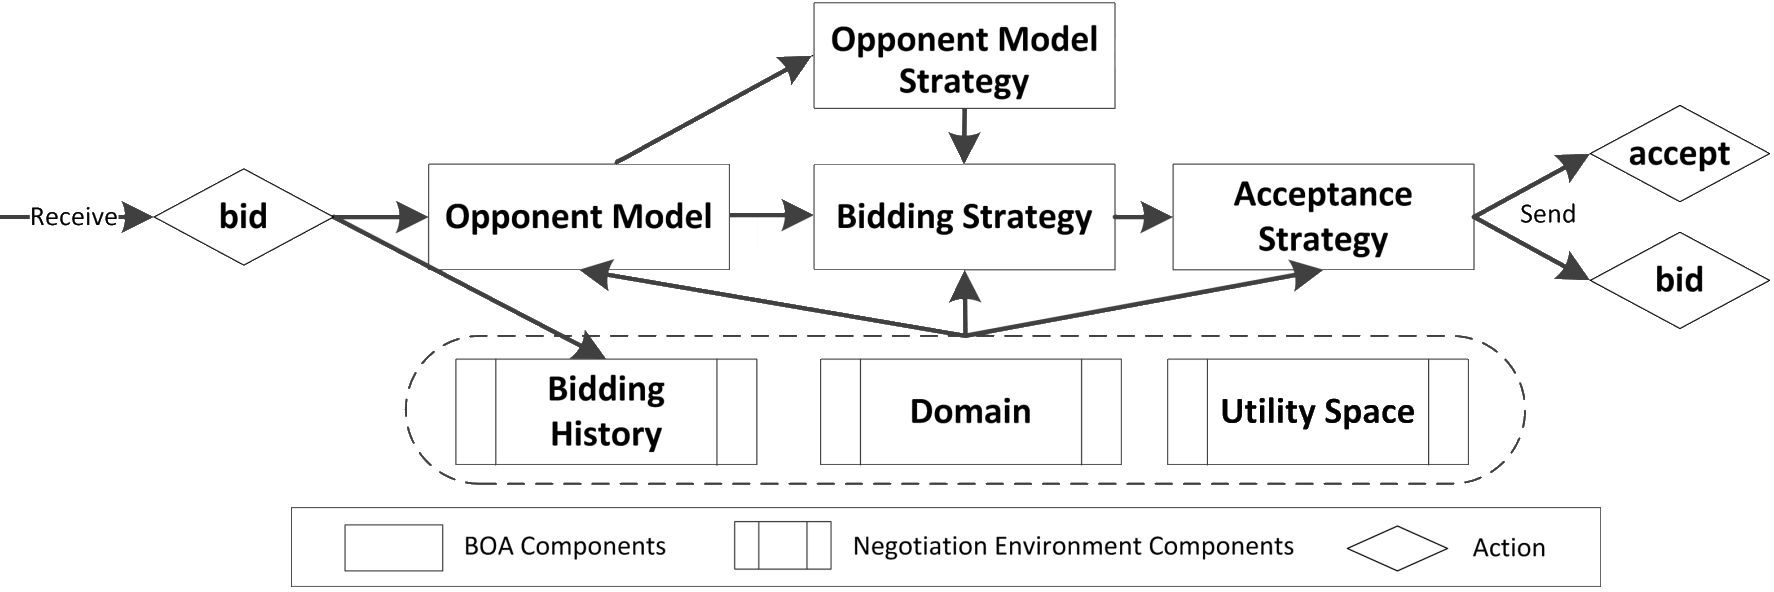
\includegraphics[width=15.0cm]{media/BOAflow.png}
	\caption{The BOA Framework Architecture.}
	\label{fig:flowchart}
\end{figure}

\FloatBarrier

\subsection{Create a BOA Party}
A boa parties can be edited in the "Boa Parties" repository tab (Figure \ref{fig:boaparties}). Right-click in the panel to add items. Select an item and right-click to remove or edit an item.   


\begin{figure}[!ht] 
	\center
	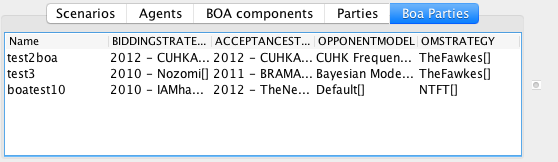
\includegraphics[width=10.0cm]{media/boacomponants.png}
	\caption{The BOA Parties repository tab.}
	\label{fig:boaparties}
\end{figure}


After you selected to add or edit a BOA party (Figure \ref{fig:editboaparty}).  Here you can select a different Offering Strategy, Acceptance Strategy, Opponent Model and Opponent Model Strategy by selecting the appropriate strategy with the combo boxes. If the strategy has parameters, the current parameter settings are shown and the respective "Change" button enables.


\begin{figure}[!ht] 
	\center
	\includegraphics[width=10.0cm]{media/EditBoaParty.png}
	\caption{Editing a BOA party.}
	\label{fig:editboaparty}
\end{figure}

If you click on the  "Change" button, another panel pops up where you can edit the parameters (Figure \ref{fig:editparameters}). You can click directly in the table to edit values.

\begin{figure}[!ht] 
	\center
	\includegraphics[width=10.0cm]{media/EditParameters.png}
	\caption{Editing the Parameters of a BOA party.}
	\label{fig:editparameters}
\end{figure}

When you have correctly set all strategies and their parameters, you can click the "OK" button in the BOA party editor (Figure  \ref{fig:editboaparty}). Then, parties with the given name are generated, one for each permutation of the range of settings you set in the parameters. For example, if you set you want parameter m to have values 0,1 and 2 and x to have values 7 and 8, there will appear 6 new parties, with settings [0,7],[0,8],[1,7],[1,8],[2,7], and [2,8]. Be careful with this generation as it is easy to create an excessive amount of boa parties this way.


\subsection{Creating BOA Components} \label{sec:creating-boa-components}
This section discusses how create your own components. An example implementation of each component is included in the ``bilateralexamples/boacomponents'' folder. The next section discusses how these components can be added to the list of available components in the BOA framework GUI. 

The \verb|bilateralexamples/boacomponents| folder contains two acceptance components:
\begin{itemize}
\item \verb|AC_Next| which  will accept an opponent bid if the utility is higher than the bid the agent is ready to present
\item \verb|AC_Uncertain| which can handle both normal and uncertain profiles.
\end{itemize}

\subsubsection{Set up a Workspace}
BOA components must be compiled before they can be loaded into Genius.
To compile a BOA component, follow the steps in (Section \ref{sec:appendix}). Then, create your BOA code into \verb|src|. For a quick start, you can copy the bilateralexamples folder into \verb|src|. Eclipse automatically compiles your BOA components into \verb|bin|.

Please refer to chapter \ref{sec:debugging} for instructions on running {\Genius} in debug mode to debug your components. 

\subsubsection{Add component to Genius}
After your component has been compiled, you need to tell Genius where to find it.
Go to the "BOA Components" tab and right click in the table. Select "Add new component". Enter the component name and click "Open". Browse to your compiled component and click "Open". Click ""Add component". After this, your component appears in the list and is ready for use.  

\subsubsection{Parameters}
All BOA components have the same mechanism to be tuned with parameters. They should have no constructor : the default empty constructor will be called. They initialize through a call to init().

The parameters and their default parameters are indicated by the component by overriding the getParameters() function. This function should return a set of $BOAparameter$ objects, each parameter having a unique name, description and default value.


\begin{table}[h]
\begin{tabular}{m{0.9\textwidth}}
\hline
\texttt{public Set<BOAparameter> getParameterSpec() }\\
 Override this function to add parameters to the module.\\
\hline
\end{tabular}
\caption{The getParameters method. Override if your component has parameters.}
\label{tab:parameters}
\end{table}


When the component is actually used, the actual values for the parameters (which may differ from the default) are passed to the init function when the component is initialized.

\subsubsection{Creating an Offering Strategy}
An offering strategy can be easily created by extending the \textit{OfferingStrategy} class. Table~\ref{tab:BOAbs} depicts the methods which need to be overridden. The \textit{init} method of the offering strategy is automatically called by the BOA framework with four parameters: the negotiation session, the opponent model, the opponent model strategy, and the parameters of the component. The negotiation session object keeps track of the negotiation state, which includes all offers made by both partiess, the timeline, the preference profile, and the domain. The parameters object specifies the parameters as specified in the GUI. In the previous section we specified the parameter $b$ for the acceptance strategy $Other - Next$ to be 0.0. In this case the party can retrieve the value of the parameter by calling \textit{parameters.get(``b'')}.

An approach often taken by many offering strategies is to first generate all possible bids. This can be efficiently done by using the \textit{SortedOutcomeSpace} class. For an example on using this class see the \textit{TimeDependent\_Offering} class in the \textit{bilateralexamples/boacomponents} directory.

\begin{table}[h]
\begin{tabular}{m{0.9\textwidth}}
\hline
\texttt{void init(NegotiationSession negotiationSession, OpponentModel opponentModel, 
	OMStrategy omStrategy, Map<String, Double> parameters)}\\
Method directly called after creating the party which should be used to initialize the component.\\
\hline
\texttt{BidDetails determineOpeningBid()}\\
Method which determines the first bid to be offered to the component.\\
\hline
\texttt{BidDetails determineNextBid()}\\
Method which determines the bids offered to the opponent after the first bid.\\
\hline
\end{tabular}
\caption{The main methods of the offering strategy component.}
\label{tab:BOAbs}
\end{table}


\subsubsection{Creating an Acceptance Condition}
This section discusses how to create an acceptance strategy class by extending the abstract class \textit{AcceptanceStrategy}. Table~\ref{tab:BOAas} depicts the two methods which need to specified.

\begin{table}[h]
\begin{tabular}{m{0.9\textwidth}}
\hline
\texttt{void init(NegotiationSession negotiationSession, OfferingStrategy offeringStrategy,
			OpponentModel opponentModel, Map<String, Double> parameters)}\\
Method directly called after creating the party which should be used to initialize the component.\\
\hline
\texttt{Actions determineAcceptability()}\\
Method which determines if the party should accept the opponent's bid (\textit{Actions.Accept}), reject it and send a counter offer (\textit{Actions.Reject}), or leave the negotiation (\textit{Actions.Break}).\\
\hline
\end{tabular}
\caption{The main methods of the acceptance strategy component.}
\label{tab:BOAas}
\end{table}

\subsubsection{Creating an Opponent Model}
This section discusses how to create an opponent model by extending the abstract class \textit{OpponentModel}. Table~\ref{tab:BOAom} provides an overview of the main methods which need to specified. For performance reasons it is recommended to use the \textit{UtilitySpace} class.

\begin{table}[h]
\begin{tabular}{m{0.9\textwidth}}
\hline
\texttt{void init(NegotiationSession negotiationSession, Map<String, Double> parameters)}\\
Method directly called after creating the party which should be used to initialize the component.\\
\hline
\texttt{double getBidEvaluation(Bid bid)}\\
Returns the estimated utility of the given bid.\\
\hline
\texttt{double updateModel(Bid bid)}\\
Updates the opponent model using the given bid.\\
\hline
\texttt{UtilitySpace getOpponentUtilitySpace()}\\
Returns the opponent's preference profile. Use the \textit{UtilitySpaceAdapter} class when not using the UtilitySpace class for the opponent's preference profile.\\
\hline
\end{tabular}
\caption{The main methods of the opponent model component.}
\label{tab:BOAom}
\end{table}

\subsubsection{Creating an Opponent Model Strategy}
This section discusses how to create an opponent model strategy by extending the abstract class \textit{OMStrategy}. Table~\ref{tab:BOAoms} provides an overview of the main methods which need to specified.

\begin{table}[h]
\begin{tabular}{m{0.9\textwidth}}
\hline
\texttt{void init(NegotiationSession negotiationSession, OpponentModel model, Map<String, Double> parameters)}\\
Method directly called after creating the party which should be used to initialize the component.\\
\hline
\texttt{BidDetails getBid(List<BidDetails> bidsInRange);}\\
This method returns a bid to be offered from a set of given similarly preferred bids by using the opponent model.\\
\hline
\texttt{boolean canUpdateOM();}\\
Determines if the opponent model may be updated this turn.\\
\hline
\end{tabular}
\caption{The main methods of the opponent model strategy component.}
\label{tab:BOAoms}
\end{table}



% DISABLED: Boa framework sessiondata is not good, it should use PersistentDataStore. 

%\subsection{SessionData}
%The BOA framework stores an object \textit{SessionData} that includes the data saved by all three components. This object is loaded and saved automatically by the BOA framework. A component can easily access the data it saved by using the \textit{loadData} method. A component can at each moment during the negotiation update the saved information by using the \textit{storeData} method, although we recommend updating the information at the end of the negotiation by using the the \textit{endSession} method. The \textit{endSession} method of each method is automatically called at the end of the negotiation to inform the component of the result obtained and should be used to update the \textit{SessionData} object before it is automatically stored.

\subsection{Advanced: Converting a BOA Party to a Party}
To convert a BOA party to a normal party you have to create a class that extends \textit{BoaParty} and override the \textit{init} method. Below is an example of a BOA party wrapped as a normal party. It's a bit hack-y because the BoaParty constructor assumes all components known  while an party often can decide this only at init time.

\begin{lstlisting}
public class SimpleBoaParty extends BoaParty {

	public SimpleBoaParty() {
		super(null, new HashMap<String, Double>(), null,
				new HashMap<String, Double>(), null,
				new HashMap<String, Double>(), null,
				new HashMap<String, Double>());
	}

	@Override
	public void init(NegotiationInfo info) {
		SessionData sessionData = null;
		if (info.getPersistentData()
				.getPersistentDataType() == PersistentDataType.SERIALIZABLE) {
			sessionData = (SessionData) info.getPersistentData().get();
		}
		if (sessionData == null) {
			sessionData = new SessionData();
		}

		negotiationSession = new NegotiationSession(sessionData,
				info.getUtilitySpace(), info.getTimeline());
		opponentModel = new MyrequencyModel();
		opponentModel.init(negotiationSession, new HashMap<String, Double>());
		omStrategy = new NullStrategy(negotiationSession);
		offeringStrategy = new MyBiddingStrategy(negotiationSession,
				opponentModel, omStrategy);

		acceptConditions = new AC_Next(negotiationSession, offeringStrategy, 1,
				0);
		// we have init'd all params here, don't call super init
	}

	@Override
	public String getDescription() {
		return "Simple BOA Party";
	}
}
\end{lstlisting}

\subsection{Advanced: Multi-Acceptance Criteria (MAC)}
The \textit{BOA framework} allows us to better explore a large space of negotiation strategies. MAC can be used to scale down the negotiation space, and thereby make it better computationally explorable.

As discussed in the introduction of this chapter, the acceptance condition determines solely if a bid should be accepted. This entails that it does not influence the bidding trace, except for when it is stopped. In fact, the only difference between \textit{BOA parties} where only the acceptance condition vary, is the time of agreement (assuming that the computational cost of the acceptance conditions are negligible).

Given this property, multiple acceptance criteria can be tested in parallel during the same negotiation trace. In practice, more than 50 variants of a simple acceptance condition as for example $\textbf{AC}_{next}$ can be tested in the same negotiation at a negligible computational cost.

To create a multi-acceptance condition component you first need to extend the class \textit{Mulit Acceptance Condition}, this gives access to the ACList which is a list of acceptance conditions to be tested in parallel. Furthermore, the method \textit{isMac} should be overwritten to return \textit{true} and the name of the components in the repository should be \textit{Multi Acceptance Criteria}. An acceptance can be added to the MAC by appending it to the AClist as shown below. 

\begin{lstlisting}[language=Java, caption={Example code for Acceptance condition}]
public class AC_MAC extends Multi_AcceptanceCondition {
	@Override
	public void init(NegotiationSession negoSession, 
			OfferingStrategy strat, OpponentModel opponentModel, 
			HashMap<String, Double> parameters) throws Exception {
		this.negotiationSession = negoSession;
		this.offeringStrategy = strat;
		outcomes = new ArrayList<OutcomeTuple> ();
		ACList = new ArrayList<AcceptanceStrategy>();
		for (int e = 0; e < 5; e++) {
			ACList.add(new AC_Next(negotiationSession, 
				offeringStrategy, 1, e * 0.01));
		}
	}
}
\end{lstlisting}




%=========================================================================================

\section{Debugging}\label{sec:debugging}
This section explains how to debug your party using Eclipse. It is assumed you set up your party already as in Chapter \ref{sec:createagent}.

You can place a breakpoint in your party (or any other place in {\Genius}) and run {\Genius} using the standard Eclipse methods (e.g. open a java file with Eclipse and click in the left border to add a breakpoint at that point).

To debug your party as it runs in Genius, right click on your project root in the Navigator (or Project explorer, whichever you use) and select Debug As.../Java Application. Then select \verb|Application - genius| and click ok.


\subsection{Source code and javadocs}
The genius core source codes and javadocs are included in the genius.jar file. But if you like you can browse and download all sources at \url{https://tracinsy.ewi.tudelft.nl/pubtrac/Genius}.

\FloatBarrier






\section{Conclusion}
This concludes the manual of {\Genius}. If you experience problems or have suggestions on how to improve {\Genius}, please send them to \url{negotiation@ii.tudelft.nl}. 

{\Genius} is actively used in academic research. If you want to use {\Genius} in your paper, please refer to \cite{Genius}.

%%%%%%%%%%%%%%%%%%%%%%%%%%%%%%%%%%%%%%%%%%%%%%%%%%%%%%%%%%%%%%%%%%%%%%%%%%%%%%%%%%%

\newpage
\section{Appendix}
This appendix describes how to set up Eclipse to create and debug your own party.

\label{sec:appendix}

\subsection{Connect Genius to Eclipse}
\label{sec:appendix-run-genius}
We expect that you installed Eclipse (Neon or higher) and Java version 8 on your computer.
\begin{enumerate}

\item Open the Eclipse Navigator with the menu Window/Show View/Navigator. You can close the Package Explorer.

\item Right click in the Navigator area and select New/Java Project. Create a new Java project. We name it \texttt{Group3assignment} but you can use any convenient name. Make sure you select "JavaSE-1.8" or equivalent to ensure your code will be java 8 compatible (Figure \ref{fig:run-genius-1}). Click Finish.

\begin{figure}[h!]
	\centering
		\includegraphics[width=0.5\textwidth]{media/dialogNewJavaProject.png}
		\caption{Create a new java project with the proper name and settings.}
	\label{fig:run-genius-1}
\end{figure}

\item Drag the genius.jar file (from your unzipped download) into the project in the Eclipse Navigator area. Select "Copy files" and press OK.

\FloatBarrier

\item{Connect \texttt{genius} Jar:
	\begin{enumerate}
		\item Right click on the \texttt{Group3assignment} icon and select "Properties".
		\item Select the Java Build Path.
		\item Select the Libraries Tab.
		\item Select "Add JARs", in the JAR Selection window (Figure \ref{fig:run-genius-3}).
		\item Open the \texttt{Group3assignment} folder and scroll down to select \texttt{genius.jar}.
		\item click a few times ok to close all dialog boxes.
	\end{enumerate}
	}
	
\begin{figure}[h!]
	\centering
		\includegraphics[width=0.6\textwidth]{media/selectjar.png}
		\caption{Attach the {\Genius} jar to the project.}
	\label{fig:run-genius-3}
\end{figure}


   
\item Now you can run G\textsc{enius} as a Java application, by launching it as a \texttt{Application} (Figure \ref{fig:startgenius}). To do this, right click on the project, select \texttt{Run As}, select \texttt{Java Application} and then in the browser select \texttt{Application - genius}.

\begin{figure}[h!]
	\centering
		\includegraphics[width=0.6\textwidth]{media/startup.png}
		\caption{Starting {\Genius} in Eclipse.}
	\label{fig:startgenius}
\end{figure}
\end{enumerate}

\FloatBarrier

\subsection{Insert example party}
To compile an example party, just drag an example folder, eg \emph{bilateralexamples}, from your unzipped genius download entirely into the src folder in Eclipse. Select "Copy files and folders" and click ok. 

You can now work with these agents in {\Genius} by adding them to the repository (see Section~\ref{sec:creating-boa-components}).

\subsection{Debugging}
Once you have Genius running in Eclipse, you can simply place a breakpoint in your party and run Genius from Eclipse in debug mode.




\bibliographystyle{plain}
\bibliography{genius}

\end{document}